\documentclass[12pt]{article}
\usepackage[ukrainian,shorthands=off]{babel}   % shorthands=off: символ " не активний (потрібно для міток "..." у TikZ всередині \zadtask)
\usepackage{fontspec}
% --- НАЛАШТУВАННЯ ШРИФТІВ ---
% Шрифти Schoolbook-*.otf лежать у корені проєкту. Шлях підбирається автоматично:
% ../ (компіляція з папки теми), ./ (корінь проєкту), ../../ (підпапки теми 28); інакше -- TeX Gyre Schola.
\newcommand{\nmtSchoolbook}[1]{\setmainfont{Schoolbook-Regular.otf}[
    Path = #1,
    BoldFont = Schoolbook-Bold.otf,
    ItalicFont = Schoolbook-Italic.otf,
    BoldItalicFont = Schoolbook-BoldItalic.otf
]}
\IfFileExists{../Schoolbook-Regular.otf}{\nmtSchoolbook{../}}{%
 \IfFileExists{./Schoolbook-Regular.otf}{\nmtSchoolbook{./}}{%
  \IfFileExists{../../Schoolbook-Regular.otf}{\nmtSchoolbook{../../}}{%
   \setmainfont{texgyreschola}[Extension=.otf, UprightFont=*-regular, BoldFont=*-bold, ItalicFont=*-italic, BoldItalicFont=*-bolditalic]}}}
\usepackage[italic]{mathastext}
\usepackage[a4paper,margin=1.8cm,bottom=2cm,top=2cm]{geometry}
\usepackage{amsmath,amssymb}
\usepackage{tikz}
\usepackage{pgfplots}
\pgfplotsset{compat=1.18}
\usepgfplotslibrary{fillbetween}
\usetikzlibrary{calc,patterns,angles,quotes,intersections,babel,3d,shapes.symbols,shapes.geometric,decorations.pathreplacing,shadings,arrows.meta,hobby}
\usepackage{xcolor,array,fancyhdr,enumitem,multicol}
\usepackage{colortbl,multirow,diagbox,needspace}
\usepackage{tcolorbox}
\tcbuselibrary{skins,breakable}
\usepackage[hidelinks]{hyperref}
% водяний знак; щоб зібрати без нього (версія для вчителів), перед \documentclass пишуть \def\nmtnowatermark{}
\ifdefined\nmtnowatermark\else
\usepackage[firstpage=false, text=@pvtr2525, scale=0.6, color=gray!12]{draftwatermark}
\fi

% --- АВТОСТИСКАННЯ: рисунок/сітка, ширша за колонку, масштабується до ширини колонки ---
\newsavebox{\nmtfitbox}
\newenvironment{nmtfit}{\begin{lrbox}{\nmtfitbox}}{\end{lrbox}%
  \ifdim\wd\nmtfitbox>\linewidth \resizebox{\linewidth}{!}{\usebox{\nmtfitbox}}\else\usebox{\nmtfitbox}\fi}
\let\nmtIncludegraphicsOrig\includegraphics
\renewcommand{\includegraphics}[2][]{\begin{nmtfit}\nmtIncludegraphicsOrig[#1]{#2}\end{nmtfit}}


\definecolor{mainGreen}{RGB}{34, 120, 64}
\definecolor{yearOrange}{RGB}{220, 100, 30}
\definecolor{yearcolor}{RGB}{220, 100, 30}
\definecolor{titleBg}{RGB}{225, 240, 220}
\definecolor{instrBg}{RGB}{255, 240, 220}
\definecolor{instrBorder}{RGB}{220, 150, 80}
\definecolor{headerblue}{RGB}{0, 102, 204}   % використовується в рисунках старої бази

\setlength{\parindent}{0pt}
\emergencystretch=1.5em

\pagestyle{fancy}
\fancyhf{}
\renewcommand{\headrulewidth}{0.4pt}
\renewcommand{\footrulewidth}{0.4pt}
\fancyhead[C]{\small\color{gray!80} Геометрія: завдання на відповідність без обчислення площ}
\fancyhead[R]{\small\color{mainGreen}\textbf{\href{https://t.me/pvtr2525}{@pvtr2525}}}
\fancyfoot[L]{\small\color{gray!80}\href{https://t.me/pvtr2525}{ТГ: @pvtr2525}}
\fancyfoot[C]{\small\color{gray!80}\thepage}
\fancyfoot[R]{\small\color{gray!80}НМТ 2022--2026}

% --- ТАБЛИЦІ ВІДПОВІДЕЙ ---
% ширина клітинки = (ширина рядка - відступи) / 5: на всю сторінку це ~3 см, у minipage поруч із рисунком таблиця стискається;
% п'ять колонок |m{w}| мають 10 відступів \tabcolsep і 6 вертикальних ліній -- тоді таблиця рівно на \linewidth
\newlength{\nmtcellw}
\newcommand{\nmtSetCell}{\setlength{\nmtcellw}{\dimexpr(\linewidth-10\tabcolsep-6\arrayrulewidth)/5\relax}}
\newcommand{\answerTable}[5]{%
\par\nopagebreak\vspace{0.15cm}
\noindent\nmtSetCell
\begin{tabular}{|*{5}{>{\centering\arraybackslash}m{\nmtcellw}|}}
\hline
\rule[-0.15cm]{0pt}{0.6cm}\textbf{А} & \rule[-0.15cm]{0pt}{0.6cm}\textbf{Б} & \rule[-0.15cm]{0pt}{0.6cm}\textbf{В} & \rule[-0.15cm]{0pt}{0.6cm}\textbf{Г} & \rule[-0.15cm]{0pt}{0.6cm}\textbf{Д} \\
\hline
\rule[-0.2cm]{0pt}{0.75cm}#1 & \rule[-0.2cm]{0pt}{0.75cm}#2 & \rule[-0.2cm]{0pt}{0.75cm}#3 & \rule[-0.2cm]{0pt}{0.75cm}#4 & \rule[-0.2cm]{0pt}{0.75cm}#5 \\
\hline
\end{tabular}
\par\vspace{0.25cm}
}
\newcommand{\answerTableTall}[5]{%
\par\nopagebreak\vspace{0.15cm}
\noindent\nmtSetCell
\begin{tabular}{|*{5}{>{\centering\arraybackslash}m{\nmtcellw}|}}
\hline
\rule[-0.2cm]{0pt}{0.7cm}\textbf{А} & \rule[-0.2cm]{0pt}{0.7cm}\textbf{Б} & \rule[-0.2cm]{0pt}{0.7cm}\textbf{В} & \rule[-0.2cm]{0pt}{0.7cm}\textbf{Г} & \rule[-0.2cm]{0pt}{0.7cm}\textbf{Д} \\
\hline
\rule[-0.45cm]{0pt}{1.2cm}#1 & \rule[-0.45cm]{0pt}{1.2cm}#2 & \rule[-0.45cm]{0pt}{1.2cm}#3 & \rule[-0.45cm]{0pt}{1.2cm}#4 & \rule[-0.45cm]{0pt}{1.2cm}#5 \\
\hline
\end{tabular}
\par\vspace{0.25cm}
}
\newcommand{\instructionBox}[1]{%
\par\vspace{0.3cm}
\begin{tcolorbox}[colback=instrBg, colframe=instrBorder, boxrule=0.6pt, arc=2pt,
    left=8pt, right=8pt, top=4pt, bottom=4pt]
\centering\small\bfseries #1
\end{tcolorbox}
\par\vspace{0.15cm}
}
\newcommand{\sectionTitle}[1]{%
\par\vspace{0.4cm}
\begin{tcolorbox}[colback=titleBg, colframe=titleBg, boxrule=0pt, arc=8pt,
    halign=center, fontupper=\Large\bfseries\color{mainGreen}]
\hyphenpenalty=10000 \exhyphenpenalty=10000 #1
\end{tcolorbox}
\par\vspace{0.3cm}
}
\newcommand{\task}[2]{\noindent\textbf{#1.}\ \ #2\par\vspace{0.2cm}}
% --- НМТ-СТИЛЬ ПОЛЕ ВІДПОВІДІ ---
\newcommand{\nmtAnswerBox}{%
\par\nopagebreak\vspace{0.2cm}\noindent
Відповідь:\ \
\begin{tabular}{@{}*{4}{|>{\centering\arraybackslash}p{0.8cm}}|@{\hspace{0.1cm}\textbf{,}\hspace{0.1cm}}*{3}{|>{\centering\arraybackslash}p{0.8cm}}|@{}}
\hline
\rule[-0.2cm]{0pt}{0.7cm} & & & & & & \\
\hline
\end{tabular}
\par\vspace{0.3cm}
}
% --- СІТКА ДЛЯ МАТЧИНГУ ---
\newsavebox{\nmtgridbox}
\newcommand{\matchingGrid}{%
    \sbox{\nmtgridbox}{\matchingGridRaw}%
    \ifdim\wd\nmtgridbox>\linewidth \resizebox{\linewidth}{!}{\usebox{\nmtgridbox}}\else\usebox{\nmtgridbox}\fi}
\newcommand{\matchingGridRaw}{%
    \begingroup
    \renewcommand{\arraystretch}{1.15}
    \setlength{\tabcolsep}{4pt}
    \footnotesize
    \begin{tabular}{r|c|c|c|c|c|}
         \multicolumn{1}{c}{} & \multicolumn{1}{c}{\textbf{А}} & \multicolumn{1}{c}{\textbf{Б}} & \multicolumn{1}{c}{\textbf{В}} & \multicolumn{1}{c}{\textbf{Г}} & \multicolumn{1}{c}{\textbf{Д}} \\ \cline{2-6}
         \textbf{1} & \phantom{X} & \phantom{X} & \phantom{X} & \phantom{X} & \phantom{X} \\ \cline{2-6}
         \textbf{2} & & & & & \\ \cline{2-6}
         \textbf{3} & & & & & \\ \cline{2-6}
    \end{tabular}
    \endgroup
}
% --- ДОДАТКОВІ МАКРОСИ ЗБІРНИКА ---
\newcommand{\taskBlock}[1]{%
\par\vspace{0.45cm}
\noindent{\color{mainGreen}\rule{\linewidth}{0.8pt}}\par\vspace{0.12cm}
\noindent{\small\bfseries\color{mainGreen}#1}\par\vspace{0.25cm}
}
\newcounter{zad}
\newcommand{\zadtask}[1]{\stepcounter{zad}\noindent\textbf{\thezad.}\ \ #1\par\nopagebreak\vspace{0.2cm}}
\newcommand{\zadnum}{\stepcounter{zad}\textbf{\thezad.}\ \ }
\newcounter{ans}
\newcommand{\ansitem}[1]{\stepcounter{ans}\noindent\textbf{\theans.}\ #1\par\vspace{0.07cm}}
% мітка року: нерозривна, притиснута праворуч; якщо не вміщається -- праворуч на новому рядку
\newcommand{\nmtyear}[1]{\unskip\nobreak\finalhyphendemerits=0 \hfill\penalty100\hskip1em\hbox{}\nobreak\hfill{\small\color{yearOrange}\mbox{\rule{0pt}{2.3ex}(НМТ~#1)}}}
% --- МАКРОС КОРОТКОГО РОЗВ'ЯЗКУ ---
\newcommand{\solution}[1]{%
\par\vspace{0.12cm}
\begin{tcolorbox}[colback=titleBg!45, colframe=mainGreen!55, boxrule=0.4pt, arc=2pt,
    left=6pt, right=6pt, top=3pt, bottom=3pt, breakable]
\footnotesize\textbf{Короткий розв'язок.}\ #1
\end{tcolorbox}
\par\vspace{0.12cm}
}
% Розв'язки й відповіді (є до завдань НМТ-2026): \showsolutionstrue -- показати, \showsolutionsfalse -- сховати
\newif\ifshowsolutions
\showsolutionsfalse
% --- ЗАГОЛОВКИ З ПУНКТАМИ КЛІКАБЕЛЬНОГО ЗМІСТУ ---
\setcounter{tocdepth}{2}
\newcommand{\chapterTitle}[1]{%
\clearpage\phantomsection\addcontentsline{toc}{section}{#1}%
\sectionTitle{#1}}
\newcommand{\typeTitle}[1]{%
\needspace{6\baselineskip}%
\phantomsection\addcontentsline{toc}{subsection}{\quad #1}%
\par\vspace{0.3cm}
\noindent{\large\bfseries\color{yearOrange}#1}\par\vspace{0.08cm}
\noindent{\color{yearOrange}\rule{\linewidth}{0.4pt}}\par\nopagebreak\vspace{0.2cm}}
\raggedbottom
% усередині одного завдання сторінка не розривається: нерозривний вертикальний проміжок
% і нерозривна межа абзаців (умова ніколи не відділяється від варіантів, рисунка чи сітки)
\newcommand{\nbvspace}[1]{\nopagebreak\vspace{#1}}
\newcommand{\nmtnobreak}{\ifvmode\penalty10000 \fi}
% --- ЄДИНИЙ МАКЕТ ЗАВДАНЬ НА ВІДПОВІДНІСТЬ ---
% мітка в колонці сталої ширини, текст -- у parbox: продовження довгого рядка
% вирівнюється під текстом, а не під міткою; відступ між пунктами однаковий скрізь
\newlength{\nmtMatchLab}\setlength{\nmtMatchLab}{1.6em}
\newlength{\nmtMatchSep}\setlength{\nmtMatchSep}{0.28cm}
\newcommand{\matchHead}[1]{\par\noindent\textit{#1}\par\nopagebreak\vspace{0.2cm}}
% шаблонний заголовок стовпця зі старого макета -- лише коли завдання не має власного \matchHead
\makeatletter\newcommand{\nmtHeadUnless}[2]{\in@{\matchHead}{#1}\ifin@\else#2\fi}\makeatother
\newcommand{\matchItem}[2]{\par\noindent\makebox[\nmtMatchLab][l]{\textbf{#1}}%
\parbox[t]{\dimexpr\linewidth-\nmtMatchLab\relax}{\raggedright #2}\par\nopagebreak\vspace{\nmtMatchSep}}
\newcommand{\ansTheme}[1]{\par\vspace{0.25cm}\noindent{\bfseries\color{mainGreen}#1}\par\vspace{0.12cm}}
\newcommand{\ansType}[1]{\par\vspace{0.1cm}\noindent{\itshape\color{yearOrange}#1}\par\vspace{0.08cm}}

% варіанти відповіді окремими рядками (довгі вирази не влазять у клітинки таблиці)
\newcommand{\answerRows}[5]{\par\nopagebreak\vspace{0.15cm}%
\matchItem{А}{#1}\matchItem{Б}{#2}\matchItem{В}{#3}\matchItem{Г}{#4}\matchItem{Д}{#5}}
\graphicspath{{./}{11. Трикутники/}{12. Паралелограм/}{13. Прямокутник/}{14. Квадрат/}{15. Ромб/}{16. Трапеція/}{17. Коло, круг і їх елементи/}}

\begin{document}
\begingroup\setcounter{zad}{0}
% --- макроси з файлів сесій НМТ-2026 (для рисунків) ---
\renewcommand{\headrulewidth}{0.4pt}
\renewcommand{\footrulewidth}{0.4pt}
\definecolor{gold}{RGB}{240, 190, 40}
\definecolor{silver}{RGB}{170, 170, 175}
\definecolor{bronze}{RGB}{190, 120, 70}
\definecolor{hexcol}{RGB}{200,110,60}
\newcommand{\hexthree}[2]{%
    \draw[hexcol, line width=1.1pt]
        ($(#1,#2)+(0:30)$) -- ($(#1,#2)+(60:30)$) -- ($(#1,#2)+(120:30)$) --
        ($(#1,#2)+(180:30)$) -- ($(#1,#2)+(240:30)$) -- ($(#1,#2)+(300:30)$) -- cycle;
}

% --- сумісність зі старою базою (діє, якщо тема не має власного визначення) ---
\providecommand{\trigStyle}[1]{#1}
\providecommand{\answerTableSmall}[5]{%
\begingroup\setlength{\tabcolsep}{2pt}\small\nmtSetCell
\begin{tabular}{|*{5}{>{\centering\arraybackslash}m{\nmtcellw}|}}
\hline
\rule[-0.2cm]{0pt}{0.6cm}\textbf{А} & \textbf{Б} & \textbf{В} & \textbf{Г} & \textbf{Д} \\
\hline
\rule[-0.4cm]{0pt}{0.9cm}#1 & \rule[-0.4cm]{0pt}{0.9cm}#2 & \rule[-0.4cm]{0pt}{0.9cm}#3 & \rule[-0.4cm]{0pt}{0.9cm}#4 & \rule[-0.4cm]{0pt}{0.9cm}#5 \\
\hline
\end{tabular}\endgroup}
\providecommand{\matchingLayout}[3]{%
    \noindent
    \begin{minipage}[t]{0.36\textwidth}\vspace{0pt}\raggedright
        #1
    \end{minipage}%
    \hfill
    \begin{minipage}[t]{0.43\textwidth}\vspace{0pt}\raggedright
        #2
    \end{minipage}%
    \hfill
    \begin{minipage}[t]{0.19\textwidth}
        \vspace{0pt}
        \begin{flushright}
        #3
        \end{flushright}
    \end{minipage}}
\providecommand{\matchingLayoutBottom}[2]{%
    \noindent
    \begin{minipage}[t]{0.48\textwidth}\vspace{0pt}\raggedright
        #1
    \end{minipage}%
    \hfill
    \begin{minipage}[t]{0.48\textwidth}\vspace{0pt}\raggedright
        #2
    \end{minipage}
    \vspace{0.5cm}
    \noindent
    \matchingGrid}
\providecommand{\answerListVertical}[5]{%
    \par\nopagebreak\vspace{0.2cm}
    \begin{itemize}[itemsep=0.4cm, leftmargin=1.5cm, labelsep=0.5cm]
        \item[\textbf{А}] #1
        \item[\textbf{Б}] #2
        \item[\textbf{В}] #3
        \item[\textbf{Г}] #4
        \item[\textbf{Д}] #5
    \end{itemize}
    \vspace{0.2cm}}

\graphicspath{{./}{11. Трикутники/}}
\setcounter{zad}{0}

\chapterTitle{Геометрія: завдання на відповідність без обчислення площ}

\noindent{\small Збірник містить \textbf{58 завдань} НМТ 2023--2026 років на встановлення відповідності з планіметрії, у яких \textit{не треба знаходити площу}: довжини відрізків, кути, радіуси кіл, периметри. Завдання зібрано з бази НМТ і згруповано за фігурою; біля кожного вказано рік. Відповіді~--- на останній сторінці.\par\vspace{0.15cm}
За роками: \mbox{2023~--- 17}, \mbox{2024~--- 13}, \mbox{2025~--- 14}, \mbox{2026~--- 14}.}\par\vspace{0.45cm}

\typeTitle{Трикутник: відрізки, висоти, радіуси кіл}

\begin{samepage}
% Завдання 19 (на відповідність, з простим рисунком TikZ)
\zadtask{Периметр рівнобедреного трикутника (див. рисунок) дорівнює 32 \textit{см}. $AB = BC = 10$ \textit{см}. До кожного відрізка \mbox{(1--3)} доберіть його довжину \mbox{(А--Д)}. \nmtyear{2023}}

\nmtnobreak
\nopagebreak\nbvspace{0.3cm}
\begin{minipage}[t]{0.55\textwidth}
\noindent
\begin{minipage}[t]{0.46\linewidth}
\matchHead{Відрізок}
\matchItem{1}{$AC$}
\matchItem{2}{висота з вершини $B$}
\matchItem{3}{радіус описаного кола}
\end{minipage}%
\hfill
\begin{minipage}[t]{0.5\linewidth}
\matchHead{Довжина відрізка}
\matchItem{А}{$6{,}25$ \textit{см}}
\matchItem{Б}{$7{,}5$ \textit{см}}
\matchItem{В}{$8$ \textit{см}}
\matchItem{Г}{$12$ \textit{см}}
\matchItem{Д}{$12{,}5$ \textit{см}}
\end{minipage}

\end{minipage}
\hfill
\begin{minipage}[t]{0.4\textwidth}\nbvspace{0pt}
\begin{flushright}
\begin{nmtfit}\begin{tikzpicture}[scale=1.6]
    % Вершини трикутника
    \coordinate (A) at (0,0);
    \coordinate (C) at (3,0);
    \coordinate (B) at (1.5,2.2);

    % Трикутник
    \draw[thick] (A) -- (B) -- (C) -- cycle;

    % Позначки рівних сторін
    \draw (0.6,1.2) -- (0.75,1.05);
    \draw (0.65,1.15) -- (0.8,1);
    \draw (2.4,1.2) -- (2.25,1.05);
    \draw (2.35,1.15) -- (2.2,1);

    % Підписи
    \node[below left] at (A) {$A$};
    \node[below right] at (C) {$C$};
    \node[above] at (B) {$B$};
\end{tikzpicture}\end{nmtfit}

\nopagebreak\nbvspace{0.3cm}
\matchingGrid
\end{flushright}
\end{minipage}
\par\penalty-20\vspace{0.25cm}
\end{samepage}

\begin{samepage}
% Завдання 33
\zadtask{На рисунку зображено прямокутний трикутник $ABC$ ($\angle C = 90°$). Точка $M$ --- середина $CB = 16$ \textit{см}. Радіус кола, описаного навколо трикутника $ABC$, дорівнює 10 \textit{см}. До кожного відрізка \mbox{(1--3)} доберіть його довжину \mbox{(А--Д)}. \nmtyear{2024}}

\nmtnobreak
\nopagebreak\nbvspace{0.3cm}
\matchingLayout{
\matchHead{Відрізок}
\matchItem{1}{$AC$}
\matchItem{2}{найбільша середня лінія трикутника $ABC$}

\nmtnobreak
\matchItem{3}{$AM$}
}{
\matchHead{Довжина відрізка}
\matchItem{А}{$10$ \textit{см}}
\matchItem{Б}{$12$ \textit{см}}
\matchItem{В}{$16$ \textit{см}}
\matchItem{Г}{$4\sqrt{11}$ \textit{см}}
\matchItem{Д}{$4\sqrt{13}$ \textit{см}}
}{
\matchingGrid
}
\hfill
\begin{minipage}[t]{0.3\textwidth}\nbvspace{0pt}
\begin{flushright}
\begin{nmtfit}\begin{tikzpicture}[scale=0.5]
    % Прямокутний трикутник
    \coordinate (A) at (0,4);
    \coordinate (B) at (4,0);
    \coordinate (C) at (0,0);

    % Середина CB
    \coordinate (M) at (2,0);

    % Трикутник
    \draw[thick] (A) -- (B) -- (C) -- cycle;

    % Прямий кут при C
    \draw (0,0.4) -- (0.4,0.4) -- (0.4,0);

    % Риски рівності на CM і MB
    \draw[thick] (0.9,-0.15) -- (0.9,0.15);
    \draw[thick] (A) -- (M);
    \draw[thick] (1.05,-0.15) -- (1.05,0.15);
    \draw[thick] (2.95,-0.15) -- (2.95,0.15);
    \draw[thick] (3.1,-0.15) -- (3.1,0.15);

    % Підписи
    \node[above left] at (A) {$A$};
    \node[right] at (B) {$B$};
    \node[below left] at (C) {$C$};
    \node[below] at (M) {$M$};
\end{tikzpicture}\end{nmtfit}
\end{flushright}
\end{minipage}
\par\penalty-20\vspace{0.25cm}
\end{samepage}

\begin{samepage}
% Завдання 32
\zadtask{У рівносторонньому трикутнику $ABC$ $AB = 24$ \textit{см}. З точки $K$, що є серединою сторони $AB$, на сторону $AC$ опущено перпендикуляр $KM$ (див. рисунок). До кожного початку речення \mbox{(1--3)} доберіть його закінчення \mbox{(А--Д)} так, щоб утворилося правильне твердження. \nmtyear{2024}}

\nmtnobreak
\nopagebreak\nbvspace{0.3cm}
\matchingLayout{
\matchHead{Початок речення}
\matchItem{1}{Відстань від точки $K$ до середини сторони $BC$}

\nmtnobreak
\matchItem{2}{Відстань від точки $M$ до прямої $BC$}

\nmtnobreak
\matchItem{3}{Сума радіусів описаного та вписаного в цей трикутник кіл}
}{
\matchHead{Закінчення речення}
\matchItem{А}{дорівнює $12$ \textit{см}.}
\matchItem{Б}{дорівнює $16$ \textit{см}.}
\matchItem{В}{дорівнює $6\sqrt{3}$ \textit{см}.}
\matchItem{Г}{дорівнює $9\sqrt{3}$ \textit{см}.}
\matchItem{Д}{дорівнює $12\sqrt{3}$ \textit{см}.}
}{
\matchingGrid
}
\hfill
\begin{minipage}[t]{0.22\textwidth}\nbvspace{0pt}
\begin{flushright}
\begin{nmtfit}\begin{tikzpicture}[scale=0.95]
    % Рівносторонній трикутник: A і C -- основа, B -- угорі (як в оригіналі)
    \coordinate (A) at (0,0);
    \coordinate (C) at (4,0);
    \coordinate (B) at (2,3.46);

    % K -- середина AB
    \coordinate (K) at (1,1.73);

    % M -- основа перпендикуляра з K на AC
    \coordinate (M) at (1,0);

    % Трикутник
    \draw[thick] (A) -- (B) -- (C) -- cycle;

    % Перпендикуляр KM
    \draw[thick] (K) -- (M);

    % Підписи
    \node[below left] at (A) {$A$};
    \node[below right] at (C) {$C$};
    \node[above] at (B) {$B$};
    \node[left] at (K) {$K$};
    \node[below] at (M) {$M$};
    \pic[draw, angle radius=0.2cm] {right angle = K--M--C};
\end{tikzpicture}\end{nmtfit}
\end{flushright}
\end{minipage}
\par\penalty-20\vspace{0.25cm}
\end{samepage}

\begin{samepage}
% Завдання 45
\zadtask{На рисунку зображено два рівні рівнобедрені трикутники $ABC$ ($AB = BC$) і $CMN$ ($CM = MN$), що лежать в одній площині. $AN = 8$ \textit{см}, $AB = 2\sqrt{17}$ \textit{см}. Узгодьте відрізок \mbox{(1--3)} із його довжиною \mbox{(А--Д)}. \nmtyear{2025}}

\nmtnobreak
\nopagebreak\nbvspace{0.3cm}
\matchingLayout{
\matchHead{Відрізок}
\matchItem{1}{Відстань від $B$ до сторони $AC$}
\matchItem{2}{$BM$}
\matchItem{3}{Відстань між серединами сторін $AB$ і $MN$}
}{
\matchHead{Довжина відрізка}
\matchItem{А}{4 \textit{см}}
\matchItem{Б}{6 \textit{см}}
\matchItem{В}{7 \textit{см}}
\matchItem{Г}{8 \textit{см}}
\matchItem{Д}{10 \textit{см}}
}{
\matchingGrid
}
\nopagebreak\nbvspace{0.3cm}
\begin{center}
\begin{nmtfit}\begin{tikzpicture}[scale=0.42]
    % AN = 8, тож AC = CN = 4; AB = BC = CM = MN = 2*sqrt17, висота 8 (точний масштаб)
    \coordinate (A) at (0,0);
    \coordinate (C) at (4,0);
    \coordinate (N) at (8,0);
    \coordinate (B) at (2,8);
    \coordinate (M) at (6,8);

    % Трикутники
    \draw[thick] (A) -- (B) -- (C) -- cycle;
    \draw[thick] (C) -- (M) -- (N) -- cycle;

    % Позначки рівних сторін
    \draw (1.34,3.915) -- (0.66,4.085);
    \draw (2.66,3.915) -- (3.34,4.085);
    \draw (5.34,3.915) -- (4.66,4.085);
    \draw (6.66,3.915) -- (7.34,4.085);

    % Підписи
    \node[below left] at (A) {$A$};
    \node[below] at (C) {$C$};
    \node[below right] at (N) {$N$};
    \node[above] at (B) {$B$};
    \node[above] at (M) {$M$};
\end{tikzpicture}\end{nmtfit}
\end{center}
\par\penalty-20\vspace{0.25cm}
\end{samepage}

\begin{samepage}
% НМТ 2026, сесія 4.06, завдання №18
\zadtask{Прямокутні рівнобедрені трикутники $ABC$ і $KMN$ є рівними (див. рисунок). Точки $K$, $C$, $N$ і $A$ лежать на прямій $AK$, причому $AN = NC = CK$. $AC = 12$~см. Установіть відповідність між відрізком \mbox{(1--3)} та його довжиною \mbox{(А--Д)}. \nmtyear{2026}\par
\nopagebreak\nbvspace{0.2cm}
\noindent
\begin{minipage}[c]{0.62\textwidth}
\begin{minipage}[t]{0.55\textwidth}
\matchHead{Відрізок}
\matchItem{1}{$AK$}
\matchItem{2}{$AB$}
\matchItem{3}{$BM$}
\end{minipage}%
\hfill
\begin{minipage}[t]{0.42\textwidth}
\matchHead{Довжина відрізка}
\matchItem{А}{$6\sqrt{2}$~см}
\matchItem{Б}{$6\sqrt{5}$~см}
\matchItem{В}{$12\sqrt{2}$~см}
\matchItem{Г}{$18$~см}
\matchItem{Д}{$24$~см}
\end{minipage}
\par\nbvspace{0.3cm}
\matchingGrid
\end{minipage}%
\hfill
\begin{minipage}[c]{0.36\textwidth}
\centering
\begin{nmtfit}\begin{tikzpicture}[scale=0.7, thick]
    \coordinate (K) at (-3,3);
    \coordinate (M) at (1,3);
    \coordinate (N) at (1,-1);
    \coordinate (C) at (-1,1);
    \coordinate (B) at (-1,-3);
    \coordinate (A) at (3,-3);
    \draw (K) -- (M) -- (N);
    \draw (C) -- (B) -- (A);
    \draw (K) -- (A);
    \draw (M) ++(-0.4,0) -- ++(0,-0.4) -- ++(0.4,0);
    \draw (B) ++(0,0.4) -- ++(0.4,0) -- ++(0,-0.4);
    \draw (-2-0.15, 2-0.15) -- (-2+0.15, 2+0.15);
    \draw (0-0.15, 0-0.15) -- (0+0.15, 0+0.15);
    \draw (2-0.15, -2-0.15) -- (2+0.15, -2+0.15);
    \fill (C) circle (2pt);
    \fill (N) circle (2pt);
    \node[above left] at (K) {$K$};
    \node[above right] at (M) {$M$};
    \node[left] at (-1.1, 0.9) {$C$};
    \node[right] at (1.1, -0.9) {$N$};
    \node[below left] at (B) {$B$};
    \node[below right] at (A) {$A$};
\end{tikzpicture}\end{nmtfit}
\end{minipage}
}
% Відповідь: 1~--~Г, 2~--~А, 3~--~Б
\ifshowsolutions\solution{$AC$~--- гіпотенуза рівнобедреного прямокутного $\triangle ABC$, тож катети $AB=BC=\dfrac{AC}{\sqrt2}=\dfrac{12}{\sqrt2}=6\sqrt2$~см (А). Оскільки $AN=NC=CK=\dfrac{AC}{2}=6$, маємо $AK=AN+NC+CK=18$~см (Г). Точка $B$ лежить на відстані катета від $C$; $BN$ обчислюється з прямокутного трикутника $BCN$ ($BC=6\sqrt2$, $CN=6$): тоді й $BM=\sqrt{BC^2+CM^2}$ дає $6\sqrt5$~см (Б). Відповідь: \textbf{1~--~Г, 2~--~А, 3~--~Б}.}\fi
\par\penalty-20
\end{samepage}

\typeTitle{Кути на рисунку}

\begin{samepage}
\noindent\zadnum \begin{minipage}[t]{0.55\textwidth}
У прямокутному трикутнику $ACB$ $\angle C = 90^\circ, \angle B = 24^\circ$. На продовжені катета $AC$ вибрано точку $K$ так, що $AK = KB$ (див. рисунок). Точка $O$ --- центр кола, описаного навколо трикутника $ACB$. До кожного кута \mbox{(1--3)} доберіть його градусну міру \mbox{(А--Д)}. \nmtyear{2023}
\end{minipage}
\hfill
\begin{minipage}[t]{0.4\textwidth}
    \nopagebreak\nbvspace{-0.3cm}
    \begin{flushright}
    \begin{nmtfit}\begin{tikzpicture}[scale=0.7]
        \coordinate (C) at (0,0);
        \coordinate (B) at (4,0);
        \coordinate (A) at (0,2); % CA < CB visually
        % K is on extension of AC downwards.
        % AK = KB. Let K = (0, y_k). A = (0, 2). B = (4, 0).
        % AK = 2 - y_k (since y_k < 0).
        % KB = sqrt(4^2 + y_k^2).
        % (2 - y_k)^2 = 16 + y_k^2
        % 4 - 4y_k + y_k^2 = 16 + y_k^2
        % -4y_k = 12 => y_k = -3.
        \coordinate (K) at (0,-3);

        \draw[thick] (K) -- (A) -- (B) -- cycle; % Triangle ABK
        \draw[thick] (K) -- (B); 
        \draw[thick] (C) -- (B); % Leg CB

        % Right angle at C
        \draw (0,0) rectangle (0.3,0.3);

        % Mark AK = KB?
        % Visual marks
        \draw[thick] ($(A)!0.5!(K)$) ++(0.15,0) -- ++(-0.3,0);
        \draw[thick] ($(K)!0.5!(B)$) ++(120:0.15) -- ++(-60:0.3);

        % Angle 24
        \pic [draw, pic text={\small $24^\circ$}, angle radius=.5cm, angle eccentricity=1.8] {angle = A--B--C};

        \node[left] at (A) {$A$};
        \node[left] at (C) {$C$};
        \node[left] at (K) {$K$};
        \node[right] at (B) {$B$};

    \end{tikzpicture}\end{nmtfit}
    \end{flushright}
\end{minipage}

\nmtnobreak
\nopagebreak\nbvspace{0.3cm}

\nmtnobreak
\matchingLayout{
\matchHead{Кут}
\matchItem{1}{$\angle BAC$}
\matchItem{2}{$\angle KBC$}
\matchItem{3}{$\angle OKB$}
}{
\matchHead{Градусна міра кута}
    \matchItem{А}{$24^\circ$}
\matchItem{Б}{$34^\circ$}
\matchItem{В}{$42^\circ$}
\matchItem{Г}{$66^\circ$}
\matchItem{Д}{$72^\circ$}
}{
    \matchingGrid
}
\par\penalty-20\vspace{0.25cm}
\end{samepage}

\begin{samepage}
\noindent\zadnum \begin{minipage}[t]{0.55\textwidth}
На катеті $BC$ прямокутного трикутника $ACB$, у якому $\angle C = 90^\circ, \angle B = 32^\circ$, вибрано точку $K$ так, що $AK = KB$ (див. рисунок). Точка $O$ --- центр кола, описаного навколо трикутника $ACB$. До кожного кута \mbox{(1--3)} доберіть його градусну міру \mbox{(А--Д)}. \nmtyear{2023}
\end{minipage}
\hfill
\begin{minipage}[t]{0.4\textwidth}
    \nopagebreak\nbvspace{-0.3cm}
    \begin{flushright}
    \begin{nmtfit}\begin{tikzpicture}[scale=0.8]
        \coordinate (C) at (0,0);
        \coordinate (A) at (0,3);
        \coordinate (B) at (5,0);

        % K on BC. AK = KB.
        % Let K = (x, 0).
        % AK^2 = x^2 + 3^2. KB^2 = (5-x)^2.
        % x^2 + 9 = 25 - 10x + x^2.
        % 10x = 16 => x = 1.6.
        \coordinate (K) at (1.6, 0);

        \draw[thick] (A) -- (C) -- (B) -- cycle;
        \draw[thick] (A) -- (K);

        % Marks AK = KB
        \draw[thick] ($(A)!0.5!(K)$) ++(150:0.15) -- ++(-30:0.3);
        \draw[thick] ($(K)!0.5!(B)$) ++(90:0.15) -- ++(-90:0.3);

        % Right angle
        \draw (0,0) rectangle (0.3,0.3);

        % Angle 32
        \pic [draw, pic text={\small $32^\circ$}, angle radius=1.0cm, angle eccentricity=1.4] {angle = A--B--C};

        \node[above] at (A) {$A$};
        \node[below] at (C) {$C$};
        \node[below] at (K) {$K$};
        \node[below] at (B) {$B$};

    \end{tikzpicture}\end{nmtfit}
    \end{flushright}
\end{minipage}

\nmtnobreak
\nopagebreak\nbvspace{0.3cm}

\nmtnobreak
\matchingLayout{
\matchHead{Кут}
\matchItem{1}{$\angle KAB$}
\matchItem{2}{$\angle KAC$}
\matchItem{3}{$\angle OKB$}
}{
\matchHead{Градусна міра кута}
    \matchItem{А}{$24^\circ$}
\matchItem{Б}{$26^\circ$}
\matchItem{В}{$32^\circ$}
\matchItem{Г}{$58^\circ$}
\matchItem{Д}{$64^\circ$}
}{
    \matchingGrid
}
\par\penalty-20\vspace{0.25cm}
\end{samepage}

\begin{samepage}
% НМТ 2026, сесія 12.06, завдання №18 --- також у темі: Коло, круг і їх елементи
\zadtask{Усередині рівнобічної трапеції $ABCD$ вибрано точку $M$, яка рівновіддалена від усіх вершин трапеції. $\angle BMC = 60^\circ$, $\angle MAD = 30^\circ$. Узгодьте кут \mbox{(1--3)} з його градусною мірою \mbox{(А--Д)}. \nmtyear{2026}\par
\nopagebreak\nbvspace{0.3cm}
\begin{minipage}[t]{0.65\textwidth}
\nopagebreak\nbvspace{0.6cm}
\begin{center}
\begin{nmtfit}\begin{tikzpicture}[scale=1, line join=round, line cap=round]
    % Центр кола (точка M)
    \coordinate (M) at (0,0);

    % Вершини трапеції (лежать на колі радіуса 2.5)
    \coordinate (B) at (120:2.5);
    \coordinate (C) at (60:2.5);
    \coordinate (A) at (210:2.5);
    \coordinate (D) at (330:2.5);

    % Малювання трапеції
    \draw[thick] (A) -- (B) -- (C) -- (D) -- cycle;

    % Відрізки від центру до вершин
    \draw[thick] (M) -- (A);
    \draw[thick] (M) -- (B);
    \draw[thick] (M) -- (C);
    \draw[thick] (M) -- (D);

    % Точка M
    \fill (M) circle (1.5pt);

    % Підписи вершин
    \node[below left=-2pt] at (A) {$A$};
    \node[above left=-2pt] at (B) {$B$};
    \node[above right=-2pt] at (C) {$C$};
    \node[below right=-2pt] at (D) {$D$};
    \node[right=2pt] at (M) {$M$};

    % Дуга та кут BMC = 60
    \draw[thick] (60:0.6) arc (60:120:0.6);
    \node at (90:0.85) {$60^{\circ}$};

    % Подвійна дуга та кут MAD = 30
    \draw[thick] ($(A) + (0:0.75)$) arc (0:30:0.75);
    \draw[thick] ($(A) + (0:0.9)$) arc (0:30:0.9);
    \node at ($(A) + (15:1.3)$) {$30^{\circ}$};

    % Позначки рівності (одинарні штрихи на бічних сторонах)
    \path (A) -- (B) node[midway, sloped] {$|$};
    \path (C) -- (D) node[midway, sloped] {$|$};

    % Позначки рівності (подвійні штрихи на відрізках до центру)
    \path (M) -- (A) node[midway, sloped] {$||$};
    \path (M) -- (B) node[midway, sloped] {$||$};
    \path (M) -- (C) node[midway, sloped] {$||$};
    \path (M) -- (D) node[midway, sloped] {$||$};
\end{tikzpicture}\end{nmtfit}
\end{center}
\end{minipage}

\nmtnobreak
\nopagebreak\nbvspace{0.2cm}
\noindent
\matchingLayout{
\matchHead{Кут}
\matchItem{1}{$\angle AMD$}
\matchItem{2}{$\angle AMB$}
\matchItem{3}{$\angle ABC$}
}{
\matchHead{Градусна міра кута}
\matchItem{А}{$90^\circ$}
\matchItem{Б}{$105^\circ$}
\matchItem{В}{$120^\circ$}
\matchItem{Г}{$135^\circ$}
\matchItem{Д}{$150^\circ$}
}{
\matchingGrid
}
}
\par\penalty-20
\end{samepage}

\begin{samepage}
% НМТ 2026, сесія 5.06, завдання №18
\zadnum На рисунку зображено правильний трикутник $ABC$ та прямокутні рівнобедрені трикутники $AKB$ і $BMC$. Установіть відповідність між кутом \mbox{(1--3)} та його градусною мірою \mbox{(А--Д)}. \nmtyear{2026}\par
\nopagebreak\nbvspace{0.3cm}
\begin{center}
\begin{nmtfit}\begin{tikzpicture}[scale=1.9, thick]
    \coordinate (A) at (0,0);
    \coordinate (C) at (2,0);
    \coordinate (B) at (1,1.732);
    \coordinate (K) at (-0.366,1.366);
    \coordinate (M) at (2.366,1.366);
    \draw[thick] (A) -- (B) -- (C) -- cycle;
    \draw[thick] (A) -- (K) -- (B);
    \draw[thick] (B) -- (M) -- (C);
    \draw[thick] (A) -- (M);
    \draw[thick] (K) -- (B);
    \pic[draw=yearOrange, line width=0.5pt, angle radius=0.3cm] {right angle = A--K--B};
    \pic[draw=yearOrange, line width=0.5pt, angle radius=0.3cm] {right angle = B--M--C};
    \node[below left, font=\scriptsize] at (A) {$A$};
    \node[above, font=\scriptsize] at (B) {$B$};
    \node[below right, font=\scriptsize] at (C) {$C$};
    \node[left, font=\scriptsize] at (K) {$K$};
    \node[right, font=\scriptsize] at (M) {$M$};
\end{tikzpicture}\end{nmtfit}
\end{center}
\nopagebreak\nbvspace{0.2cm}
\noindent
\matchingLayout{
\matchHead{Кут}
\matchItem{1}{$\angle ACM$}
\matchItem{2}{$\angle KBM$}
\matchItem{3}{$\angle KAM$}
}{
\matchHead{Градусна міра}
\matchItem{А}{$75^\circ$}
\matchItem{Б}{$90^\circ$}
\matchItem{В}{$105^\circ$}
\matchItem{Г}{$135^\circ$}
\matchItem{Д}{$150^\circ$}
}{
\matchingGrid
}
\par\nbvspace{0.5cm}
% Відповідь: 1~--~В, 2~--~Д, 3~--~А
\ifshowsolutions\solution{Кути правильного трикутника по $60^\circ$, а в прямокутних рівнобедрених трикутниках $AKB$, $BMC$ кути при основі по $45^\circ$. Тоді $1$: $\angle ACM=\angle ACB+\angle BCM=60^\circ+45^\circ=105^\circ$ (В); $2$: $\angle KBM=\angle KBA+\angle ABC+\angle CBM=45^\circ+60^\circ+45^\circ=150^\circ$ (Д); $3$: $\angle KAM=75^\circ$ (А). Відповідь: \textbf{1~--~В, 2~--~Д, 3~--~А}.}\fi
\par\penalty-20
\end{samepage}

\begin{samepage}
% НМТ 2026, сесія 10.06, завдання №18
\zadtask{На рисунку зображено ромб $ABCD$ й рівнобедрений трикутник $AKD$, які лежать в одній площині. $\angle BAD = 50^\circ$, $\angle AKD = 40^\circ$. Узгодьте кут \mbox{(1--3)} з його градусною мірою \mbox{(А--Д)}. \nmtyear{2026}\par
\nopagebreak\nbvspace{0.3cm}
\begin{center}
\begin{nmtfit}\begin{tikzpicture}[scale=0.55, thick, line join=round]
    \coordinate (A) at (0,0);
    \coordinate (D) at (3.5,0);
    \coordinate (B) at (2.25,2.68);
    \coordinate (C) at (5.75,2.68);
    \coordinate (K) at (1.75,-4.8);
    \draw (A) -- (B) -- (C) -- (D) -- cycle;
    \draw (A) -- (D);
    \draw (A) -- (K) -- (D);
    % мітки рівності бічних сторін
    \draw ($(A)!0.5!(K)$) ++(-0.12,-0.04) -- ++(0.24,0.08);
    \draw ($(D)!0.5!(K)$) ++(-0.12,0.04) -- ++(0.24,-0.08);
    \pic[draw, angle radius=0.55cm, pic text={$50^\circ$}, angle eccentricity=1.7, font=\scriptsize] {angle = D--A--B};
    \pic[draw, angle radius=0.8cm, pic text={$40^\circ$}, angle eccentricity=1.45, font=\scriptsize] {angle = D--K--A};
    \node[left] at (A) {$A$};
    \node[above left] at (B) {$B$};
    \node[above right] at (C) {$C$};
    \node[right] at (D) {$D$};
    \node[below] at (K) {$K$};
\end{tikzpicture}\end{nmtfit}
\end{center}
\nopagebreak\nbvspace{0.2cm}
\noindent
\matchingLayout{
\matchHead{Кут}
\matchItem{1}{$\angle KAB$}
\matchItem{2}{$\angle ABC$}
\matchItem{3}{$\angle KDC$}
}{
\matchHead{Градусна міра кута}
\matchItem{А}{$110^\circ$}
\matchItem{Б}{$120^\circ$}
\matchItem{В}{$130^\circ$}
\matchItem{Г}{$150^\circ$}
\matchItem{Д}{$160^\circ$}
}{
\matchingGrid
}
}
\par\penalty-20
\end{samepage}

\begin{samepage}
% НМТ 2026, сесія 8.06, завдання №18
\zadtask{На рисунку зображено рівні паралелограми $ABCD$ і $AKMD$. $BD \perp AB$. $\angle BAD = 65^\circ$. Установіть відповідність між кутом \mbox{(1--3)} та його градусною мірою \mbox{(А--Д)}. \nmtyear{2026}\par
\nopagebreak\nbvspace{0.3cm}
\begin{center}
\begin{nmtfit}\begin{tikzpicture}[scale=0.85, thick, line join=round]
    \coordinate (A) at (0,0);
    \coordinate (D) at (5,0);
    \coordinate (B) at (0.893, 1.915); % AB = AD cos 65°, тож BD ⟂ AB
    \coordinate (C) at (5.893, 1.915);
    \coordinate (K) at (0.893, -1.915);
    \coordinate (M) at (5.893, -1.915);

    \draw (-1,0) -- (7,0); % Line AD extends
    \draw (A) -- (B) -- (C) -- (D);
    \draw (A) -- (K) -- (M) -- (D);
    \draw (B) -- (D);

    \pic[draw, angle radius=0.5cm, pic text=$65^\circ$, angle eccentricity=1.7, font=\scriptsize] {angle = D--A--B};
    \pic[draw, angle radius=0.3cm] {right angle = A--B--D};

    \node[above left] at (A) {$A$};
    \node[above left] at (B) {$B$};
    \node[above right] at (C) {$C$};
    \node[above right] at (D) {$D$};
    \node[below left] at (K) {$K$};
    \node[below right] at (M) {$M$};
\end{tikzpicture}\end{nmtfit}
\end{center}
\nopagebreak\nbvspace{0.2cm}
\noindent
\matchingLayout{
\matchHead{Кут}
\matchItem{1}{$\angle ABC$}
\matchItem{2}{$\angle CDM$}
\matchItem{3}{$\angle BDM$}
}{
\matchHead{Градусна міра}
\matchItem{А}{$115^\circ$}
\matchItem{Б}{$125^\circ$}
\matchItem{В}{$130^\circ$}
\matchItem{Г}{$140^\circ$}
\matchItem{Д}{$150^\circ$}
}{
\matchingGrid
}
}
\par\penalty-20
\end{samepage}

\typeTitle{Коло: центральний і вписаний кути, дотична}

\begin{samepage}
\noindent\zadnum \begin{minipage}[t]{0.55\textwidth}
На рисунку зображено коло з центром у точці $O$, $AB$ --- діаметр цього кола. Пряма $a$ --- дотична до цього кола, що перетинає продовження діаметра $AB$ у точці $K$, $C$ --- точка дотику. Установіть відповідність між величиною \mbox{(1--3)} та її значенням \mbox{(А--Д)}, якщо дуга $AC = 130^\circ$. \nmtyear{2023}
\end{minipage}
\hfill
\begin{minipage}[t]{0.4\textwidth}
    \nopagebreak\nbvspace{-0.3cm}
    \begin{flushright}
    \begin{nmtfit}\begin{tikzpicture}[scale=0.9]
        \coordinate (O) at (0,0);
        \draw[thick] (O) circle (1.5cm);
        \coordinate (A) at (-1.5,0);
        \coordinate (B) at (1.5,0);
        % дуга AC = 130°, тож ∠COB = 50°; дотична в C перетинає пряму AB у K: OK = R / cos 50°
        \coordinate (C) at (50:1.5);
        \coordinate (K) at (2.334,0);
        \coordinate (L) at (-0.568,2.435);

        \draw[thick] (A) -- (K);
        \draw[thick] (L) -- (C);
        \draw[thick] (C) -- (K) node[midway, above right] {$a$};
        \draw[thick] (O) -- (C);

        % дуга AC
        \draw[very thick] (A) arc (180:50:1.5);

        \node[left] at (A) {$A$};
        \node[below left] at (B) {$B$};
        \node[below] at (O) {$O$};
        \node[below right] at (K) {$K$};
        \node[above right] at (C) {$C$};

        \fill (O) circle (1.5pt);
        \fill (A) circle (1.5pt);
        \fill (B) circle (1.5pt);
        \fill (K) circle (1.5pt);
        \fill (C) circle (1.5pt);
    \end{tikzpicture}\end{nmtfit}
    \end{flushright}
\end{minipage}

\nmtnobreak
\nopagebreak\nbvspace{0.3cm}

\nmtnobreak
\matchingLayout{
\matchHead{Величина}
\matchItem{1}{дуга $CB$}
\matchItem{2}{$\angle CKA$}
\matchItem{3}{$\angle ABC$}
}{
\matchHead{Значення величини}
    \matchItem{А}{$30^\circ$}
\matchItem{Б}{$40^\circ$}
\matchItem{В}{$50^\circ$}
\matchItem{Г}{$65^\circ$}
\matchItem{Д}{$70^\circ$}
}{
    \matchingGrid
}
\par\penalty-20\vspace{0.25cm}
\end{samepage}

\begin{samepage}
\noindent\zadnum \begin{minipage}[t]{0.55\textwidth}
Точка $O$ --- центр кола, зображеного на рисунку. До цього кола проведено дотичну $KB$, $B$ --- точка дотику. На колі вибрано точки $A$ і $C$ так, що $AB = BC$, $\angle ABC = 50^\circ$. Установіть відповідність між кутом \mbox{(1--3)} та його градусною мірою \mbox{(А--Д)}. \nmtyear{2024}
\end{minipage}
\hfill
\begin{minipage}[t]{0.4\textwidth}
    \nopagebreak\nbvspace{-0.3cm}
    \begin{flushright}
    \begin{nmtfit}\begin{tikzpicture}[scale=0.7]
        \coordinate (O) at (0,0);
        \draw[thick] (O) circle (1.5cm);

        % B at top (90 deg)
        \coordinate (B) at (90:1.5);
        \coordinate (K) at (-2.5, 1.5);
        \draw[thick] (K) -- (2.5, 1.5); % Tangent line

        % Inscribed isosceles triangle ABC. AB=BC.
        % Angle ABC = 50.
        % Arc AC corresponds to 50? No, inscribed angle B=50 means Arc AC = 100.
        % Remaining arc = 260. Arc AB = Arc BC = 130.
        % B is at 90. A is at 90+130 = 220. C is at 90-130 = -40 (320).
        \coordinate (A) at (220:1.5);
        \coordinate (C) at (320:1.5);

        \draw[thick] (A) -- (B) -- (C);
        \draw[thick] (A) -- (O);
        \draw[thick] (C) -- (O);

        % Angle 50
        \pic [draw, pic text={\scriptsize $50^\circ$}, angle radius=0.4cm, angle eccentricity=1.8] {angle = A--B--C};

        % Marks for AB = BC
        \draw[thick] ($(A)!0.5!(B)$) ++(160:0.1) -- ++(-20:0.2);
        \draw[thick] ($(B)!0.5!(C)$) ++(20:0.1) -- ++(-160:0.2);

        \node[above] at (K) {$K$};
        \node[above] at (B) {$B$};
        \node[below left] at (A) {$A$};
        \node[below right] at (C) {$C$};
        \node[below] at (O) {$O$};

        \fill (O) circle (1.5pt);
        \fill (A) circle (1.5pt);
        \fill (B) circle (1.5pt);
        \fill (C) circle (1.5pt);

    \end{tikzpicture}\end{nmtfit}
    \end{flushright}
\end{minipage}

\nmtnobreak
\nopagebreak\nbvspace{0.3cm}

\nmtnobreak
\matchingLayout{
\matchHead{Кут}
\matchItem{1}{$\angle AOC$}
\matchItem{2}{$\angle BOC$}
\matchItem{3}{$\angle KBA$}
}{
\matchHead{Градусна міра кута}
    \matchItem{А}{$50^\circ$}
\matchItem{Б}{$65^\circ$}
\matchItem{В}{$100^\circ$}
\matchItem{Г}{$90^\circ$}
\matchItem{Д}{$130^\circ$}
}{
    \matchingGrid
}
\par\penalty-20\vspace{0.25cm}
\end{samepage}

\typeTitle{Квадрат}

\begin{samepage}
\noindent\zadnum \begin{minipage}[t]{0.55\textwidth}
На рисунку зображено квадрат $ABCD$. На сторонах $AD$ і $BC$ вибрано точки $K$ і $M$ так, що $AK = 4$ \textit{см}, $MC = 10$ \textit{см}, $KM = DM$. До кожної величини \mbox{(1--3)} доберіть її значення \mbox{(А--Д)}. \nmtyear{2023}
\end{minipage}
\hfill
\begin{minipage}[t]{0.4\textwidth}
    \nopagebreak\nbvspace{-0.3cm}
    \begin{flushright}
    \begin{nmtfit}\begin{tikzpicture}[scale=0.15]
        % Розрахунок: нехай сторона a.
        % K(4,0), M(a-10, a), D(a,0).
        % KM^2 = (a-10-4)^2 + a^2 = (a-14)^2 + a^2.
        % DM^2 = 10^2 + a^2.
        % (a-14)^2 = 100 => a-14 = 10 (бо сторона > 14) => a=24.
        % AK=4 (масштаб), сторона 24.

        \def\side{24}
        \coordinate (A) at (0,0);
        \coordinate (B) at (0,\side);
        \coordinate (C) at (\side,\side);
        \coordinate (D) at (\side,0);

        \coordinate (K) at (4,0);
        \coordinate (M) at (14,\side); % 24 - 10 = 14

        \draw[thick] (A) -- (B) -- (C) -- (D) -- cycle;
        \draw[thick] (K) -- (M) -- (D);

        % Позначки рівності
        \draw ($(K)!0.5!(M)$) ++(-0.5,0.5) -- ++(1,-1);
        \draw ($(D)!0.5!(M)$) ++(-0.5,0.5) -- ++(1,-1);

        \node[below left] at (A) {$A$};
        \node[above left] at (B) {$B$};
        \node[above right] at (C) {$C$};
        \node[below right] at (D) {$D$};
        \node[below] at (K) {$K$};
        \node[above] at (M) {$M$};
    \end{tikzpicture}\end{nmtfit}
    \end{flushright}
\end{minipage}

\nmtnobreak
\nopagebreak\nbvspace{0.3cm}

\nmtnobreak
\matchingLayout{
\matchHead{Величина}
\matchItem{1}{довжина сторони квадрата $ABCD$}
\matchItem{2}{довжина відрізка $DM$}
\matchItem{3}{відстань від середини відрізка $DM$ до прямої $AB$}
}{
\matchHead{Значення величини}
    \matchItem{А}{24 \textit{см}}
\matchItem{Б}{25 \textit{см}}
\matchItem{В}{19 \textit{см}}
\matchItem{Г}{18 \textit{см}}
\matchItem{Д}{26 \textit{см}}
}{
    \matchingGrid
}
\par\penalty-20\vspace{0.25cm}
\end{samepage}

\begin{samepage}
\noindent\zadnum \begin{minipage}[t]{0.55\textwidth}
На рисунку зображено квадрат $ABCD$, площа якого $144$ \textit{см}$^2$. Точки $K$ і $M$ --- середини сторін $BC$ і $CD$ відповідно. До кожного відрізка \mbox{(1--3)} доберіть його довжину \mbox{(А--Д)}. \nmtyear{2024}
\end{minipage}
\hfill
\begin{minipage}[t]{0.4\textwidth}
    \nopagebreak\nbvspace{-0.3cm}
    \begin{flushright}
    \begin{nmtfit}\begin{tikzpicture}[scale=0.35]
        \coordinate (A) at (0,0);
        \coordinate (B) at (0,10);
        \coordinate (C) at (10,10);
        \coordinate (D) at (10,0);

        \coordinate (K) at (5,10);
        \coordinate (M) at (10,5);

        \draw[thick] (A) -- (B) -- (C) -- (D) -- cycle;
        \draw[thick] (K) -- (M);
        \draw[thick] (A) -- (K); % Для краси, хоча в умові не питають, але на рисунку є лінії

        % Позначки середин
        \draw (2.5, 9.8) -- (2.5, 10.2);
        \draw (7.5, 9.8) -- (7.5, 10.2);

        \draw (9.8, 7.5) -- (10.2, 7.5);
        \draw (9.8, 2.5) -- (10.2, 2.5);

        \node[below left] at (A) {$A$};
        \node[above left] at (B) {$B$};
        \node[above right] at (C) {$C$};
        \node[below right] at (D) {$D$};
        \node[above] at (K) {$K$};
        \node[right] at (M) {$M$};

        \fill (K) circle (5pt);
        \fill (M) circle (5pt);
    \end{tikzpicture}\end{nmtfit}
    \end{flushright}
\end{minipage}

\nmtnobreak
\nopagebreak\nbvspace{0.3cm}

\nmtnobreak
\matchingLayout{
\matchHead{Відрізок}
\matchItem{1}{сторона квадрата}
\matchItem{2}{$KM$}
\matchItem{3}{відстань від точки $A$ до центра кола, описаного навколо трикутника $KMC$}
}{
\matchHead{Довжина відрізка}
    \matchItem{А}{6 \textit{см}}
\matchItem{Б}{$6\sqrt{2}$ \textit{см}}
\matchItem{В}{12 \textit{см}}
\matchItem{Г}{$8\sqrt{2}$ \textit{см}}
\matchItem{Д}{$9\sqrt{2}$ \textit{см}}
}{
    \matchingGrid
}
\par\penalty-20\vspace{0.25cm}
\end{samepage}

\begin{samepage}
% Завдання 35
\zadtask{На рисунку зображено квадрат $ABCD$ і прямокутний трикутник $KBC$ ($\angle B = 90°$), що лежать в одній площині. Периметр квадрата $ABCD$ дорівнює 24 \textit{см}, середня лінія трапеції $AKCD$ дорівнює 10 \textit{см}. До кожного відрізка \mbox{(1--3)} доберіть його довжину \mbox{(А--Д)}. \nmtyear{2024}}

\nmtnobreak
\nopagebreak\nbvspace{0.3cm}
\matchingLayout{
\matchHead{Відрізок}
\matchItem{1}{$BK$}
\matchItem{2}{$KC$}
\matchItem{3}{відстань між центрами кіл, описаних навколо квадрата $ABCD$ та трикутника $KBC$}
}{
\matchHead{Довжина відрізка}
\matchItem{А}{$6$ \textit{см}}
\matchItem{Б}{$7$ \textit{см}}
\matchItem{В}{$8$ \textit{см}}
\matchItem{Г}{$9$ \textit{см}}
\matchItem{Д}{$10$ \textit{см}}
}{
\matchingGrid
}
\hfill
\begin{minipage}[t]{0.3\textwidth}\nbvspace{0pt}
\begin{flushright}
\begin{nmtfit}\begin{tikzpicture}[scale=0.45]
    % Квадрат ABCD (A внизу ліворуч, за годинниковою)
    \coordinate (A) at (0,0);
    \coordinate (B) at (0,4);
    \coordinate (C) at (4,4);
    \coordinate (D) at (4,0);

    % Точка K над B
    \coordinate (K) at (0,8);

    % Квадрат
    \draw[thick] (A) -- (B) -- (C) -- (D) -- cycle;

    % Трикутник KBC
    \draw[thick] (K) -- (B);
    \draw[thick] (K) -- (C);

    % Прямий кут при B
    \draw (0,4.4) -- (0.4,4.4) -- (0.4,4);

    % Підписи
    \node[below left] at (A) {$A$};
    \node[left] at (B) {$B$};
    \node[right] at (C) {$C$};
    \node[below right] at (D) {$D$};
    \node[above left] at (K) {$K$};
\end{tikzpicture}\end{nmtfit}
\end{flushright}
\end{minipage}
\par\penalty-20\vspace{0.25cm}
\end{samepage}

\begin{samepage}
\noindent\zadnum \begin{minipage}[t]{0.55\textwidth}
На рисунку зображено квадрат $ABCD$. На стороні $BC$ вибрано точку $K$, так що $KC = 4$ \textit{см}. Точка $M$ --- середина відрізка $AK$. Пряма, що проходить через точку $M$, паралельна стороні $BC$, і перетинає $AB$ та $CD$ в точках $N$ і $P$ відповідно. $NM = 6$ \textit{см}. Узгодьте відрізок \mbox{(1--3)} із його довжиною \mbox{(А--Д)}. \nmtyear{2025}
\end{minipage}
\hfill
\begin{minipage}[t]{0.4\textwidth}
    \nopagebreak\nbvspace{-0.3cm}
    \begin{flushright}
    \begin{nmtfit}\begin{tikzpicture}[scale=0.25]
        % Розрахунок: NM = (AB - 4)/2? Ні.
        % Нехай сторона a. K(a-4, a). A(0,0). M((a-4)/2, a/2).
        % N(0, a/2). NM = (a-4)/2. 
        % (a-4)/2 = 6 => a-4=12 => a=16.
        % Сторона 16. KC=4. BK=12.

        \def\side{16}
        \coordinate (A) at (0,0);
        \coordinate (B) at (0,\side);
        \coordinate (C) at (\side,\side);
        \coordinate (D) at (\side,0);

        \coordinate (K) at (12,\side); % KC=4
        \coordinate (M) at (6, 8); % Середина AK (A(0,0), K(12,16)) -> (6,8)

        \coordinate (N) at (0,8);
        \coordinate (P) at (\side,8);

        \draw[thick] (A) -- (B) -- (C) -- (D) -- cycle;
        \draw[thick] (A) -- (K);
        \draw[thick] (N) -- (P);

        % Позначки рівності AM=MK
        \draw ($(A)!0.5!(M)$) ++(-0.5,0.5) -- ++(1,-1);
        \draw ($(M)!0.5!(K)$) ++(-0.5,0.5) -- ++(1,-1);

        \node[below left] at (A) {$A$};
        \node[above left] at (B) {$B$};
        \node[above right] at (C) {$C$};
        \node[below right] at (D) {$D$};
        \node[above] at (K) {$K$};
        \node[left] at (N) {$N$};
        \node[right] at (P) {$P$};
        \node[above left] at (M) {$M$};

        \fill (M) circle (10pt);
        \fill (K) circle (10pt);
        \fill (N) circle (10pt);
        \fill (P) circle (10pt);
    \end{tikzpicture}\end{nmtfit}
    \end{flushright}
\end{minipage}

\nmtnobreak
\nopagebreak\nbvspace{0.3cm}

\nmtnobreak
\matchingLayout{
\matchHead{Відрізок}
\matchItem{1}{$AB$}
\matchItem{2}{$MP$}
\matchItem{3}{$AK$}
}{
\matchHead{Довжина відрізка}
    \matchItem{А}{10 \textit{см}}
\matchItem{Б}{12 \textit{см}}
\matchItem{В}{16 \textit{см}}
\matchItem{Г}{18 \textit{см}}
\matchItem{Д}{20 \textit{см}}
}{
    \matchingGrid
}
\par\penalty-20\vspace{0.25cm}
\end{samepage}

\begin{samepage}
\noindent\zadnum \begin{minipage}[t]{0.55\textwidth}
На стороні $BC$ квадрата $ABCD$ вибрано точку $K$ так, що $BK = KC$. Діагональ $BD$ квадрата і відрізок $AK$ перетинаються в точці $M$. Периметр квадрата $ABCD$ дорівнює $120$ \textit{см}. Узгодьте відрізок \mbox{(1--3)} із його довжиною \mbox{(А--Д)}. \nmtyear{2025}
\end{minipage}
\hfill
\begin{minipage}[t]{0.4\textwidth}
    \nopagebreak\nbvspace{-0.3cm}
    \begin{flushright}
    \begin{nmtfit}\begin{tikzpicture}[scale=0.12]
        % P=120 -> сторона 30.
        % BK=KC=15.
        \coordinate (A) at (0,0);
        \coordinate (B) at (0,30);
        \coordinate (C) at (30,30);
        \coordinate (D) at (30,0);
        \coordinate (K) at (15,30);

        \draw[thick] (A) -- (B) -- (C) -- (D) -- cycle;
        \draw[thick] (A) -- (K);
        \draw[thick] (B) -- (D);

        \coordinate (M) at (intersection of A--K and B--D);

        % Позначки рівності BK=KC
        \draw (7.5, 29) -- (7.5, 31);
        \draw (22.5, 29) -- (22.5, 31);

        \node[below left] at (A) {$A$};
        \node[above left] at (B) {$B$};
        \node[above right] at (C) {$C$};
        \node[below right] at (D) {$D$};
        \node[above] at (K) {$K$};
        \node[right] at (M) {$M$};

        \fill (M) circle (15pt);
        \fill (K) circle (15pt);
    \end{tikzpicture}\end{nmtfit}
    \end{flushright}
\end{minipage}

\nmtnobreak
\nopagebreak\nbvspace{0.3cm}

\nmtnobreak
\matchingLayout{
\matchHead{Відрізок}
\matchItem{1}{$BK$}
\matchItem{2}{$BD$}
\matchItem{3}{$MD$}
}{
\matchHead{Довжина відрізка}
    \matchItem{А}{$12\sqrt{2}$ \textit{см}}
\matchItem{Б}{15 \textit{см}}
\matchItem{В}{$20\sqrt{2}$ \textit{см}}
\matchItem{Г}{$18\sqrt{2}$ \textit{см}}
\matchItem{Д}{$30\sqrt{2}$ \textit{см}}
}{
    \matchingGrid
}
\par\penalty-20\vspace{0.25cm}
\end{samepage}

\begin{samepage}
% НМТ 2026, сесія 30.05, завдання №16 --- основна тема: Квадрат
\zadtask{На рисунку зображено квадрат $ABCD$ та рівнобедрений прямокутний трикутник $KBC$ (прямий кут при вершині $K$), які мають спільну сторону $BC$. Точка $M$~--- середина сторони $CD$. Довжина ламаної $BADM$ дорівнює $20$. Установіть відповідність між величинами \mbox{(1--3)} та їхніми значеннями \mbox{(А--Д)}. \nmtyear{2026}\par
\nopagebreak\nbvspace{0.3cm}
\begin{center}
\begin{nmtfit}\begin{tikzpicture}[scale=0.75, thick]
    \coordinate (A) at (0,0);
    \coordinate (B) at (0,4);
    \coordinate (C) at (4,4);
    \coordinate (D) at (4,0);
    \coordinate (K) at (2,6);
    \coordinate (Mid) at (4,2);
    \draw[thick] (A) -- (B) -- (C) -- (D) -- cycle;
    \draw[thick] (B) -- (K) -- (C);
    \fill (Mid) circle (2pt);
    \node[below left] at (A) {$A$};
    \node[above left] at (B) {$B$};
    \node[above right] at (C) {$C$};
    \node[below right] at (D) {$D$};
    \node[above] at (K) {$K$};
    \node[right] at (Mid) {$M$};
\end{tikzpicture}\end{nmtfit}
\end{center}
\nopagebreak\nbvspace{0.2cm}
\noindent
\matchingLayout{
\matchHead{Величина}
\matchItem{1}{довжина сторони квадрата}
\matchItem{2}{відстань від точки $K$ до прямої $AD$}
\matchItem{3}{довжина відрізка $KM$}
}{
\matchHead{Значення}
\matchItem{А}{$12$}
\matchItem{Б}{$10$}
\matchItem{В}{$4\sqrt{3}$}
\matchItem{Г}{$4\sqrt{5}$}
\matchItem{Д}{$8$}
}{
\matchingGrid
}
}
% Відповідь: 1~--~Д, 2~--~А, 3~--~Г
\ifshowsolutions\solution{Нехай сторона квадрата $a$. Ламана $BADM=BA+AD+DM=a+a+\dfrac a2=\dfrac{5a}{2}=20$, звідки $a=8$ (\textbf{1}~--~Д). Висота трикутника до $BC$ дорівнює $\dfrac a2=4$, тож відстань від $K$ до $AD$: $a+\dfrac a2=12$ (\textbf{2}~--~А). У координатах $K(4;12)$, $M(8;4)$: $KM=\sqrt{4^2+8^2}=\sqrt{80}=4\sqrt5$ (\textbf{3}~--~Г). Відповідь: \textbf{1~--~Д, 2~--~А, 3~--~Г}.}\fi
\par\penalty-20
\end{samepage}

\begin{samepage}
% НМТ 2026, сесія 9.06, завдання №18
\zadtask{На рисунку зображено квадрат $ABCD$, діагональ якого дорівнює $8\sqrt{2}$~см. Установіть відповідність між відрізком \mbox{(1--3)} та його довжиною \mbox{(А--Д)}. \nmtyear{2026}\par
\nopagebreak\nbvspace{0.3cm}
\begin{center}
\begin{nmtfit}\begin{tikzpicture}[scale=0.7, thick, line join=round]
    \coordinate (A) at (0,0);
    \coordinate (B) at (0,4);
    \coordinate (C) at (4,4);
    \coordinate (D) at (4,0);
    \draw (A) -- (B) -- (C) -- (D) -- cycle;
    \node[below left] at (A) {$A$};
    \node[above left] at (B) {$B$};
    \node[above right] at (C) {$C$};
    \node[below right] at (D) {$D$};
\end{tikzpicture}\end{nmtfit}
\end{center}
\nopagebreak\nbvspace{0.2cm}
\noindent
\matchingLayout{
\matchHead{Відрізок}
\matchItem{1}{відстань між серединами сторін $AB$ і $AD$}
\matchItem{2}{радіус кола, уписаного в квадрат $ABCD$}
\matchItem{3}{медіана трикутника $ABC$, проведена з вершини $A$}
}{
\matchHead{Довжина відрізка}
\matchItem{А}{$2\sqrt{2}$~см}
\matchItem{Б}{$4$~см}
\matchItem{В}{$4\sqrt{2}$~см}
\matchItem{Г}{$8$~см}
\matchItem{Д}{$4\sqrt{5}$~см}
}{
\matchingGrid
}
}
\par\penalty-20
\end{samepage}

\typeTitle{Прямокутник}

\begin{samepage}
% === ЗАВДАННЯ 1 (Повтор з минулого файлу) ===
\noindent\zadnum \begin{minipage}[t]{0.55\textwidth}
Прямокутник $ABCD$, паралелограм $BKMC$ та трапеція $DCMN$ лежать в одній площині, точки $K$, $C$ та $D$ належать одній прямій (див. рисунок). $AB = 5$ \textit{см}, $AD = 12$ \textit{см}, $BK = 13$ \textit{см}. До кожної величини \mbox{(1--3)} доберіть її значення \mbox{(А--Д)}. \nmtyear{2023}
\end{minipage}
\hfill
\begin{minipage}[t]{0.4\textwidth}
    \nopagebreak\nbvspace{-0.3cm}
    \begin{flushright}
    \begin{nmtfit}\begin{tikzpicture}[scale=0.55]
        \coordinate (A) at (0,0);
        \coordinate (B) at (0,2);
        \coordinate (C) at (4.8,2);
        \coordinate (D) at (4.8,0);
        \coordinate (K) at (4.8,4.6);
        \coordinate (M) at (9.6,4.6);
        \coordinate (N) at (9.6,0);

        \draw[thick] (A) -- (B) -- (C) -- (D) -- cycle;
        \draw[thick] (B) -- (K) -- (M) -- (C);
        \draw[thick] (D) -- (N) -- (M);

        \draw (0,0.4) -- (0.4,0.4) -- (0.4,0);

        \node[left] at (0,1) {\small 5 \textit{см}};
        \node[below] at (2.4,0) {\small 12 \textit{см}};
        \node[above left] at (1.6,3.3) {\small 13 \textit{см}};

        \node[below left] at (A) {$A$};
        \node[above left] at (B) {$B$};
        \node[below right] at (C) {$C$};
        \node[below] at (D) {$D$};
        \node[above] at (K) {$K$};
        \node[above] at (M) {$M$};
        \node[below right] at (N) {$N$};
    \end{tikzpicture}\end{nmtfit}
    \end{flushright}
\end{minipage}

\nmtnobreak
\nopagebreak\nbvspace{0.3cm}

\nmtnobreak
\matchingLayout{
\matchHead{Величина}
\matchItem{1}{діагональ $ABCD$}
\matchItem{2}{відстань від $K$ до $AN$}
\matchItem{3}{висота трапеції $DCMN$}
}{
\matchHead{Значення}
    \matchItem{А}{10 \textit{см}}
\matchItem{Б}{12 \textit{см}}
\matchItem{В}{13 \textit{см}}
\matchItem{Г}{17 \textit{см}}
\matchItem{Д}{5 \textit{см}}
}{
    \matchingGrid
}
\par\penalty-20\vspace{0.25cm}
\end{samepage}

\begin{samepage}
% === ЗАВДАННЯ 4 (Середини сторін K і M) ===
\noindent\zadnum \begin{minipage}[t]{0.55\textwidth}
На рисунку зображено прямокутник $ABCD$. Точки $K$ і $M$ --- відповідно середини сторін $AB$ і $BC$, $AB = 12$ \textit{см}, $MC = 8$ \textit{см}. До кожного відрізка \mbox{(1--3)} доберіть його довжину \mbox{(А--Д)}. \nmtyear{2023}
\end{minipage}
\hfill
\begin{minipage}[t]{0.4\textwidth}
    \nopagebreak\nbvspace{-0.3cm}
    \begin{flushright}
    \begin{nmtfit}\begin{tikzpicture}[scale=0.15]
        % AB=12, BC=16 (MC=8 => BC=16)
        % A(0,0) - ні, нехай B буде верхній лівий, як зазвичай A внизу.
        % За рисунком: A внизу зліва. B зверху зліва.
        \coordinate (A) at (0,0);
        \coordinate (B) at (0,12);
        \coordinate (C) at (16,12);
        \coordinate (D) at (16,0);

        \coordinate (K) at (0,6); % Середина AB
        \coordinate (M) at (8,12); % Середина BC (8, 12)

        \draw[thick] (A) -- (B) -- (C) -- (D) -- cycle;
        \draw[thick] (A) -- (K) -- (M) -- (C); % Лінія на рисунку йде від A до K, потім до M, потім C?
        % На рисунку просто точки. Проведемо лінію AK і MC для візуалізації, як на скріншоті.
        % На скріншоті відрізки: AK з'єднано з M? Ні.
        % Просто позначено рівність відрізків.

        % Позначки рівності
        \draw (-0.5,3) -- (0.5,3); % AK
        \draw (-0.5,9) -- (0.5,9); % KB
        \draw[thick] (A)  -- (C);
        \draw (4,11.5) -- (4,12.5); \draw (4.2,11.5) -- (4.2,12.5); % BM
        \draw (12,11.5) -- (12,12.5); \draw (12.2,11.5) -- (12.2,12.5); % MC

        \node[below left] at (A) {$A$};
        \node[above left] at (B) {$B$};
        \node[above right] at (C) {$C$};
        \node[below right] at (D) {$D$};
        \node[left] at (K) {$K$};
        \node[above] at (M) {$M$};

        \fill (K) circle (10pt);
        \fill (M) circle (10pt);
    \end{tikzpicture}\end{nmtfit}
    \end{flushright}
\end{minipage}

\nmtnobreak
\nopagebreak\nbvspace{0.3cm}

\nmtnobreak
\matchingLayout{
\matchHead{Відрізок}
\matchItem{1}{$BC$}
\matchItem{2}{діаметр кола, описаного навколо прямокутника $ABCD$}
\matchItem{3}{відстань від точки $D$ до середини $KM$}
}{
\matchHead{Довжина відрізка}
    \matchItem{А}{10 \textit{см}}
\matchItem{Б}{15 \textit{см}}
\matchItem{В}{16 \textit{см}}
\matchItem{Г}{18 \textit{см}}
\matchItem{Д}{20 \textit{см}}
}{
    \matchingGrid
}
\par\penalty-20\vspace{0.25cm}
\end{samepage}

\begin{samepage}
% === ЗАВДАННЯ 6 (Два прямокутники, L-форма) ===
\noindent\zadnum \begin{minipage}[t]{0.55\textwidth}
Прямокутники $ABCD$ і $DKLM$ є рівними (див. рисунок). $AD = 6$, $DM = 8$. Установіть відповідність між величиною \mbox{(1--3)} та її значенням \mbox{(А--Д)}. \nmtyear{2023}
\end{minipage}
\hfill
\begin{minipage}[t]{0.4\textwidth}
    \nopagebreak\nbvspace{-0.3cm}
    \begin{flushright}
    \begin{nmtfit}\begin{tikzpicture}[scale=0.35]
        % D - спільна вершина (0,0)
        % ABCD лівий: A(-6,0), B(-6,8), C(0,8), D(0,0). (AD=6, AB=8)
        % DKLM правий: D(0,0), K(0,6), L(8,6), M(8,0). (DM=8, DK=6)

        \coordinate (D) at (0,0);
        \coordinate (A) at (-6,0);
        \coordinate (B) at (-6,8);
        \coordinate (C) at (0,8);

        \coordinate (M) at (8,0);
        \coordinate (L) at (8,6);
        \coordinate (K) at (0,6);

        \draw[thick] (A) -- (B) -- (C) -- (K) -- (L) -- (M) -- (A); % Зовнішній контур
        \draw[thick] (C) -- (D) -- (K); % Спільна лінія
        \draw[thick] (D) -- (B); % Діагональ BD
        \draw[thick] (D) -- (L); % Діагональ DL

        \node[below left] at (A) {$A$};
        \node[above left] at (B) {$B$};
        \node[above right] at (C) {$C$};
        \node[below] at (D) {$D$};
        \node[below] at (M) {$M$};
        \node[above right] at (L) {$L$};
        \node[above right] at (K) {$K$};
    \end{tikzpicture}\end{nmtfit}
    \end{flushright}
\end{minipage}

\nmtnobreak
\nopagebreak\nbvspace{0.3cm}

\nmtnobreak
\matchingLayout{
\matchHead{Величина}
\matchItem{1}{$\sin \angle MDL$}
\matchItem{2}{$\tg \angle ABD$}
\matchItem{3}{$\cos \angle BDL$}
}{
\matchHead{Значення величини}
    \matchItem{А}{0,6}
\matchItem{Б}{0,75}
\matchItem{В}{0,8}
\matchItem{Г}{0}
\matchItem{Д}{1}
}{
    \matchingGrid
}
\par\penalty-20\vspace{0.25cm}
\end{samepage}

\begin{samepage}
\noindent\zadnum \begin{minipage}[t]{0.55\textwidth}
Прямокутник $ABKM$ складається з квадрата $ABCD$ та прямокутника $DCKM$ (див. рисунок). Периметр квадрата $ABCD$ дорівнює $40$ \textit{см}, $CM = 26$ \textit{см}. Узгодьте відрізок \mbox{(1--3)} із його довжиною \mbox{(А--Д)}. \nmtyear{2025}
\end{minipage}
\hfill
\begin{minipage}[t]{0.4\textwidth}
    \nopagebreak\nbvspace{-0.3cm}
    \begin{flushright}
    \begin{nmtfit}\begin{tikzpicture}[scale=0.15]
        % Square ABCD perimeter 40 -> side 10.
        % CM = 26. In rect DCKM, side CD=10. CM is diagonal.
        % DM = sqrt(26^2 - 10^2) = 24.
        % Total width AM = 10 + 24 = 34.

        \coordinate (A) at (0,0);
        \coordinate (B) at (0,10);
        \coordinate (C) at (10,10);
        \coordinate (D) at (10,0);

        \coordinate (K) at (34,10);
        \coordinate (M) at (34,0);

        \draw[thick] (A) -- (B) -- (K) -- (M) -- cycle;
        \draw[thick] (D) -- (C); % Separator

        \node[below left] at (A) {$A$};
        \node[above left] at (B) {$B$};
        \node[above] at (C) {$C$};
        \node[below] at (D) {$D$};
        \node[above right] at (K) {$K$};
        \node[below right] at (M) {$M$};
    \end{tikzpicture}\end{nmtfit}
    \end{flushright}
\end{minipage}

\nmtnobreak
\nopagebreak\nbvspace{0.3cm}

\nmtnobreak
\matchingLayout{
\matchHead{Відрізок}
\matchItem{1}{Сторона квадрата $ABCD$}
\matchItem{2}{$CK$}
\matchItem{3}{Відстань між центром квадрата і точкою перетину діагоналей прямокутника $ABKM$}
}{
\matchHead{Довжина відрізка}
    \matchItem{А}{10 \textit{см}}
\matchItem{Б}{12 \textit{см}}
\matchItem{В}{16 \textit{см}}
\matchItem{Г}{17 \textit{см}}
\matchItem{Д}{24 \textit{см}}
}{
    \matchingGrid
}
\par\penalty-20\vspace{0.25cm}
\end{samepage}

\begin{samepage}
% НМТ 2026, сесія 15.06, завдання №18
\zadtask{На рисунку точки $K$, $L$, $M$ та $N$~--- середини сторін $AB$, $BC$, $CD$ та $AD$ прямокутника $ABCD$ відповідно. $AB = 12$~см, $BC = 16$~см. Точка $P$~--- середина відрізка $KN$. Установіть відповідність між відрізком \mbox{(1--3)} та його довжиною \mbox{(А--Д)}. \nmtyear{2026}\par
\nopagebreak\nbvspace{0.3cm}
\begin{center}
\begin{nmtfit}\begin{tikzpicture}[scale=0.55, thick, line join=round]
    \coordinate (A) at (0,0);
    \coordinate (B) at (0,12);
    \coordinate (C) at (16,12);
    \coordinate (D) at (16,0);
    \coordinate (K) at (0,6);
    \coordinate (L) at (8,12);
    \coordinate (M) at (16,6);
    \coordinate (N) at (8,0);
    \coordinate (P) at (4,3);
    \draw (A) -- (B) -- (C) -- (D) -- cycle;
    \draw (K) -- (L) -- (M) -- (N) -- cycle;
    \fill (P) circle (3pt);
    \draw (K)--(N);
    \path (K) -- (N) node[midway, sloped] {\footnotesize $|$};
    \node[below left] at (A) {$A$};
    \node[above left] at (B) {$B$};
    \node[above right] at (C) {$C$};
    \node[below right] at (D) {$D$};
    \node[left] at (K) {$K$};
    \node[above] at (L) {$L$};
    \node[right] at (M) {$M$};
    \node[below] at (N) {$N$};
    \node[above left, font=\scriptsize] at (P) {$P$};
\end{tikzpicture}\end{nmtfit}
\end{center}
\nopagebreak\nbvspace{0.2cm}
\noindent
\matchingLayout{
\matchHead{Відрізок}
\matchItem{1}{відстань від точки $P$ до сторони $BC$}
\matchItem{2}{відстань від точки $P$ до середини $MN$}
\matchItem{3}{відстань від точки $P$ до вершини $C$}
}{
\matchHead{Довжина відрізка}
\matchItem{А}{$8$~см}
\matchItem{Б}{$9$~см}
\matchItem{В}{$12$~см}
\matchItem{Г}{$15$~см}
\matchItem{Д}{$16$~см}
}{
\matchingGrid
}
}
% Відповідь: 1--Б, 2--А, 3--Г
\par\penalty-20
\end{samepage}

\begin{samepage}
% НМТ 2026, сесія 3.06, завдання №18 --- основна тема: Прямокутник
\zadnum На рисунку зображено прямокутник $ABCD$ та рівнобедрений трикутник $DKM$ ($DK = KM$). Пряма, що містить діагональ $AC$ прямокутника, проходить через точку $K$. $AB = 16$ см, $AD = 12$ см, $DM = 2AD$. Установіть відповідність між відрізком \mbox{(1--3)} та його довжиною \mbox{(А--Д)}. \nmtyear{2026}\par
\nopagebreak\nbvspace{0.3cm}
\begin{center}
\begin{nmtfit}\begin{tikzpicture}[scale=0.17, thick]
    \coordinate (A) at (0,0);
    \coordinate (B) at (0,16);
    \coordinate (Cc) at (12,16);
    \coordinate (D) at (12,0);
    \coordinate (M) at (36,0);
    \coordinate (K) at (24,32);
    \draw[thick] (A) -- (B) -- (Cc) -- (D) -- cycle;
    \draw[thick] (A) -- (M);
    \draw[thick] (D) -- (K) -- (M);
    \draw[thick] (A) -- (K);
    \fill (K) circle (3pt); \node[above, font=\scriptsize] at (K) {$K$};
    \node[below left, font=\scriptsize] at (A) {$A$};
    \node[above left, font=\scriptsize] at (B) {$B$};
    \node[above, font=\scriptsize] at (Cc) {$C$};
    \node[below, font=\scriptsize] at (D) {$D$};
    \node[below right, font=\scriptsize] at (M) {$M$};
\end{tikzpicture}\end{nmtfit}
\end{center}
\nopagebreak\nbvspace{0.2cm}
\noindent
\matchingLayout{
\matchHead{Початок речення}
\matchItem{1}{Довжина відрізка $AM$ дорівнює}
\matchItem{2}{Відстань від точки $K$ до прямої $AM$ дорівнює}
\matchItem{3}{Довжина відрізка $CK$ дорівнює}
}{
\matchHead{Закінчення}
\matchItem{А}{$20$ см}
\matchItem{Б}{$24$ см}
\matchItem{В}{$32$ см}
\matchItem{Г}{$36$ см}
\matchItem{Д}{$48$ см}
}{
\matchingGrid
}
% Відповідь: 1~--~Г, 2~--~В, 3~--~А
\ifshowsolutions\solution{$AM=AD+DM=12+2\cdot12=36$ см~--- \textbf{Г}. Нехай $H$~--- основа висоти рівнобедреного $\triangle DKM$ з вершини $K$; вона ділить $DM$ навпіл, тож $DH=12$, а $AH=AD+DH=24$. Оскільки $K$ лежить на прямій $AC$, прямокутні $\triangle ADC$ і $\triangle AHK$ подібні (спільний кут $A$, прямі кути при $D$ і $H$): $KH=CD\cdot\dfrac{AH}{AD}=16\cdot\dfrac{24}{12}=32$ см~--- \textbf{В}. З тієї самої подібності $AK=2\,AC$, де $AC=\sqrt{12^2+16^2}=20$, тож $CK=AK-AC=40-20=20$ см~--- \textbf{А}. Відповідь: \textbf{1~--~Г, 2~--~В, 3~--~А}.}\fi
\par\penalty-20
\end{samepage}

\typeTitle{Прямокутник і кола}

\begin{samepage}
% === ЗАВДАННЯ 5 (Коло і півколо) ===
\noindent\zadnum \begin{minipage}[t]{0.6\textwidth}
У прямокутник $ABCD$ вписано коло із центром в точці $O$, яке дотикається до сторін $AB$, $BC$ і $AD$, та півколо з діаметром $CD$ (див. рисунок). Коло й півколо мають лише одну спільну точку. $AB = 8$ \textit{см}. До кожного початку речення \mbox{(1--3)} доберіть його закінчення \mbox{(А--Д)} так, щоб утворилося правильне твердження. \nmtyear{2023}
\end{minipage}
\hfill
\begin{minipage}[t]{0.35\textwidth}
    \nopagebreak\nbvspace{-0.3cm}
    \begin{flushright}
    \begin{nmtfit}\begin{tikzpicture}[scale=0.3]
        % AB=8. Коло R=4. Центр O(4,4).
        % BC=12. Півколо на CD. R=4. Центр (12,4).
        % Дотикаються в точці (8,4).

        \coordinate (A) at (0,0);
        \coordinate (B) at (0,8);
        \coordinate (C) at (12,8);
        \coordinate (D) at (12,0);
        \coordinate (O) at (4,4);

        \draw[thick] (A) -- (B) -- (C) -- (D) -- cycle;

        % Коло
        \draw[thick] (O) circle (4cm);

        % Півколо (дуга від C до D зліва)
        \draw[thick] (C) arc (90:270:4cm);

        \node[below left] at (A) {$A$};
        \node[above left] at (B) {$B$};
        \node[above] at (C) {$C$};
        \node[below right] at (D) {$D$};
        \node at (O) {$\cdot$};
        \node[below right] at (O) {$O$};
    \end{tikzpicture}\end{nmtfit}
    \end{flushright}
\end{minipage}

\nmtnobreak
\nopagebreak\nbvspace{0.3cm}

\nmtnobreak
\matchingLayout{
\matchHead{Початок речення}
\matchItem{1}{Довжина сторони $BC$}
\matchItem{2}{Довжина відрізка $OC$}
\matchItem{3}{Відстань від середини відрізка $AO$ до прямої $CD$}
}{
\matchHead{Закінчення речення}
    \matchItem{А}{дорівнює 10 \textit{см}.}
\matchItem{Б}{дорівнює 12 \textit{см}.}
\matchItem{В}{дорівнює 16 \textit{см}.}
\matchItem{Г}{дорівнює $4\sqrt{5}$ \textit{см}.}
\matchItem{Д}{дорівнює $4\sqrt{3}$ \textit{см}.}
}{
    \matchingGrid
}
\par\penalty-20\vspace{0.25cm}
\end{samepage}

\begin{samepage}
\noindent\zadnum \begin{minipage}[t]{0.55\textwidth}
На рисунку зображено прямокутник $ABCD$ та два кола. Перше коло з центром у точці $O_1$, описане навколо цього прямокутника, друге коло з центром у точці $O_2$, довжиною $16\pi$ \textit{см}, дотикається до сторін $AB$, $BC$ та $AD$. $BC = 30$ \textit{см}. До кожного початку речення \mbox{(1--3)} доберіть його закінчення \mbox{(А--Д)} так, щоб утворилося правильне твердження. \nmtyear{2024}
\end{minipage}
\hfill
\begin{minipage}[t]{0.4\textwidth}
    \nopagebreak\nbvspace{-0.3cm}
    \begin{flushright}
    \begin{nmtfit}\begin{tikzpicture}[scale=0.12]
        % Circle 2 length 16pi -> R=8. Diameter 16.
        % Touches AB, BC, AD -> Height AB = 16.
        % Width BC = 30.
        \def\w{30}
        \def\h{16}
        \coordinate (A) at (0,0);
        \coordinate (B) at (0,\h);
        \coordinate (C) at (\w,\h);
        \coordinate (D) at (\w,0);

        % Center O2: r=8 from AB, r=8 from AD. (8,8)
        \coordinate (O2) at (8,8);

        % Center O1: Midpoint of rect (15,8)
        \coordinate (O1) at (15,8);

        % Circumcircle radius: sqrt(15^2+8^2) = 17.

        % Draw Circumcircle (O1) - Green
        \draw[thick, green!60!black] (O1) circle (17);

        % Draw Inscribed-like Circle (O2) - Orange
        \draw[thick, orange!80!black] (O2) circle (8);

        % Draw Rectangle
        \draw[thick] (A) -- (B) -- (C) -- (D) -- cycle;

        % Points
        \fill (O1) circle (15pt) node[right] {$O_1$};
        \fill (O2) circle (15pt) node[left] {$O_2$};

        % Labels
        \node[below left] at (A) {$A$};
        \node[above left] at (B) {$B$};
        \node[above right] at (C) {$C$};
        \node[below right] at (D) {$D$};
        \node[above] at (15, \h) {30 \textit{см}};
    \end{tikzpicture}\end{nmtfit}
    \end{flushright}
\end{minipage}

\nmtnobreak
\nopagebreak\nbvspace{0.3cm}

\nmtnobreak
\matchingLayout{
\matchHead{Початок речення}
\matchItem{1}{Довжина сторони $AB$ дорівнює}
\matchItem{2}{Довжина радіуса кола, описаного навколо прямокутника $ABCD$ дорівнює}
\matchItem{3}{Довжина відрізка $O_1O_2$ дорівнює}
}{
\matchHead{Закінчення речення}
    \matchItem{А}{7 \textit{см}.}
\matchItem{Б}{9 \textit{см}.}
\matchItem{В}{12 \textit{см}.}
\matchItem{Г}{16 \textit{см}.}
\matchItem{Д}{17 \textit{см}.}
}{
    \matchingGrid
}
\par\penalty-20\vspace{0.25cm}
\end{samepage}

\begin{samepage}
\noindent\zadnum \begin{minipage}[t]{0.55\textwidth}
На рисунку зображено прямокутник $ABCD$ та два кола. Перше коло з центром у точці $O_1$ описано навколо цього прямокутника. Площа круга, обмеженого колом з центром у точці $O_1$, дорівнює $625\pi$ \textit{см}$^2$. Друге коло з центром у точці $O_2$ дотикається до сторін $AB$, $BC$ та $AD$. $AB = 30$ \textit{см}. Узгодьте початок речення \mbox{(1--3)} із його закінченням \mbox{(А--Д)} так, щоб утворилося правильне твердження. \nmtyear{2025}
\end{minipage}
\hfill
\begin{minipage}[t]{0.4\textwidth}
    \nopagebreak\nbvspace{-0.3cm}
    \begin{flushright}
    \begin{nmtfit}\begin{tikzpicture}[scale=0.1]
        % Circumcircle Area 625pi -> R=25. Diameter AC=50.
        % AB=30. BC = sqrt(50^2 - 30^2) = 40.
        % O2 touches AB, BC, AD -> Diameter = AB = 30. Radius r=15.

        \coordinate (A) at (0,0);
        \coordinate (B) at (0,30);
        \coordinate (C) at (40,30);
        \coordinate (D) at (40,0);

        % O1 center of rect (20, 15)
        \coordinate (O1) at (20,15);

        % O2 center of inscribed-like (15, 15)
        \coordinate (O2) at (15,15);

        % Draw Green Circumcircle (R=25)
        \draw[green!60!black] (O1) circle (25);

        % Draw Orange Circle (R=15)
        \draw[orange!80!black] (O2) circle (15);

        \draw[thick] (A) -- (B) -- (C) -- (D) -- cycle;

        \fill (O1) circle (15pt) node[above right] {$O_1$};
        \fill (O2) circle (15pt) node[above left] {$O_2$};

        \node[below left] at (A) {$A$};
        \node[above left] at (B) {$B$};
        \node[above right] at (C) {$C$};
        \node[below right] at (D) {$D$};
    \end{tikzpicture}\end{nmtfit}
    \end{flushright}
\end{minipage}

\nmtnobreak
\nopagebreak\nbvspace{0.3cm}

\nmtnobreak
\matchingLayout{
\matchHead{Початок речення}
\matchItem{1}{Відстань від $O_2$ до сторони $BC$ дорівнює}
\matchItem{2}{Довжина сторони $AD$ дорівнює}
\matchItem{3}{Довжина відрізка $O_1O_2$ дорівнює}
}{
\matchHead{Закінчення речення}
    \matchItem{А}{5 \textit{см}.}
\matchItem{Б}{10 \textit{см}.}
\matchItem{В}{15 \textit{см}.}
\matchItem{Г}{25 \textit{см}.}
\matchItem{Д}{40 \textit{см}.}
}{
    \matchingGrid
}
\par\penalty-20\vspace{0.25cm}
\end{samepage}

\begin{samepage}
% Завдання 47
\zadtask{Коло із центром у точці $O$ дотикається трьох сторін прямокутника $ABCD$ (див. рисунок). Вершина $K$ прямокутного рівнобедреного трикутника $AKB$ належить колу. $AB = 12$ \textit{см}. Доберіть до кожного початку речення \mbox{(1--3)} його закінчення \mbox{(А--Д)} так, щоб утворилося правильне твердження. \nmtyear{2025}}

\nmtnobreak
\nopagebreak\nbvspace{0.3cm}
\matchingLayout{
\matchHead{Початок речення}
\matchItem{1}{Довжина радіуса $OK$ кола дорівнює}
\matchItem{2}{Довжина відрізка $BK$ дорівнює}
\matchItem{3}{Відстань від точки $O$ до вершини $A$ дорівнює}
}{
\matchHead{Закінчення речення}
\matchItem{А}{6 \textit{см}.}
\matchItem{Б}{8 \textit{см}.}
\matchItem{В}{$6\sqrt{2}$ \textit{см}.}
\matchItem{Г}{$6\sqrt{5}$ \textit{см}.}
\matchItem{Д}{18 \textit{см}.}
}{
\matchingGrid
}
\nopagebreak\nbvspace{0.3cm}
\begin{center}
\begin{nmtfit}\begin{tikzpicture}[scale=1]
    % Прямокутник ABCD
    \coordinate (A) at (0,0);
    \coordinate (B) at (0,4);
    \coordinate (C) at (6,4);
    \coordinate (D) at (6,0);

    % Центр кола O (на AD, праворуч)
    \coordinate (O) at (4,2);

    % Точка K (на колі, де дотикається трикутник)
    \coordinate (K) at (2,2);

    % Прямокутник
    \draw[thick] (A) -- (B) -- (C) -- (D) -- cycle;

    % Коло
    \draw[thick] (O) circle (2);

    % Трикутник AKB
    \draw[thick] (A) -- (K) -- (B);

    % Діагоналі трикутника (позначки рівних сторін)
    \draw (0.85,0.85) -- (1.15,1.15);
    \draw (0.85,3.15) -- (1.15,2.85);

    % Прямий кут при K
    \pic[draw, angle radius=0.3cm] { right angle = A--K--B};

    % Підписи
    \node[below left] at (A) {$A$};
    \node[above left] at (B) {$B$};
    \node[above right] at (C) {$C$};
    \node[below right] at (D) {$D$};
    \node[right] at (K) {$K$};
    \node[above] at (4.3,2) {$O$};
    \fill (O) circle (2pt);
\end{tikzpicture}\end{nmtfit}
\end{center}
\par\penalty-20\vspace{0.25cm}
\end{samepage}

\begin{samepage}
% НМТ 2026, сесія 16.06, завдання №18 --- також у темі: Коло, круг і їх елементи
\zadtask{На рисунку зображено прямокутник $ABCD$, у який вписано коло з центром у точці $O$, що дотикається до сторін $BC$ й $AD$, та два півкола, побудованих на сторонах $AB$ і $CD$ як на діаметрах, що мають лише одну спільну точку з колом. $BC = 12$~см. Установіть відповідність між відрізком \mbox{(1--3)} та його довжиною \mbox{(А--Д)}. \nmtyear{2026}}\par
\nopagebreak\nbvspace{0.3cm}
\noindent
\begin{minipage}[c]{0.52\textwidth}
\begin{minipage}[t]{0.48\textwidth}
\matchHead{Відрізок}
\matchItem{1}{радіус кола}
\matchItem{2}{$CD$}
\matchItem{3}{$AO$}
\end{minipage}
\hfill
\begin{minipage}[t]{0.48\textwidth}
\matchHead{Довжина відрізка}
\matchItem{А}{$3$~см}
\matchItem{Б}{$4$~см}
\matchItem{В}{$3\sqrt{3}$~см}
\matchItem{Г}{$6$~см}
\matchItem{Д}{$3\sqrt{5}$~см}
\end{minipage}
\nopagebreak\nbvspace{0.4cm}

\matchingGrid
\end{minipage}%
\hfill
\begin{minipage}[c]{0.45\textwidth}
\centering
\begin{nmtfit}\begin{tikzpicture}[scale=0.55, thick, line join=round]
    \coordinate (A) at (0,0);
    \coordinate (B) at (0,6);
    \coordinate (C) at (12,6);
    \coordinate (D) at (12,0);

    \draw (A) rectangle (C);

    % Півкола
    \draw (0,0) arc (-90:90:3);
    \draw (12,6) arc (90:270:3);

    % Коло в центрі
    \draw (6,3) circle (3);
    \fill (6,3) circle (2.5pt) node[right=2pt] {$O$};

    \node[below left] at (A) {$A$};
    \node[above left] at (B) {$B$};
    \node[above right] at (C) {$C$};
    \node[below right] at (D) {$D$};
\end{tikzpicture}\end{nmtfit}
\end{minipage}
% Відповідь: 1--А; 2--Г; 3--Д
\par\penalty-20
\end{samepage}

\begin{samepage}
% НМТ 2026, сесія 2.06, завдання №18 --- також у темі: Коло, круг і їх елементи
\zadtask{Прямокутник $ABCD$ і коло з центром $O$ розташовані так, що коло дотикається до середин бічних сторін $AB$ і $CD$ та перетинає сторону $BC$ у точках $K$ і $M$ (див. рисунок). Відомо, що $BK = 3$ см, $BM = 27$ см. Установіть відповідність між відрізком \mbox{(1--3)} та його довжиною \mbox{(А--Д)}. \nmtyear{2026}\par
\nopagebreak\nbvspace{0.3cm}
\begin{center}
\begin{nmtfit}\begin{tikzpicture}[scale=0.2, thick]
    \coordinate (A) at (0,0);
    \coordinate (B) at (0,18);
    \coordinate (C) at (30,18);
    \coordinate (D) at (30,0);
    \coordinate (O) at (15,9);
    \coordinate (K) at (3,18);
    \coordinate (M) at (27,18);
    \draw[thick] (A) -- (B) -- (C) -- (D) -- cycle;
    \draw[thick, mainGreen] (O) circle (15);
    \fill (O) circle (4pt); \node[below right] at (O) {$O$};
    \fill (K) circle (4pt); \node[above] at (K) {$K$};
    \fill (M) circle (4pt); \node[above] at (M) {$M$};
    \node[below left] at (A) {$A$};
    \node[above left] at (B) {$B$};
    \node[above right] at (C) {$C$};
    \node[below right] at (D) {$D$};
\end{tikzpicture}\end{nmtfit}
\end{center}
\nopagebreak\nbvspace{0.2cm}
\noindent
\matchingLayout{
\matchHead{Відрізок}
\matchItem{1}{$KM$}
\matchItem{2}{$KO$}
\matchItem{3}{$AB$}
}{
\matchHead{Довжина}
\matchItem{А}{$3$ см}
\matchItem{Б}{$15$ см}
\matchItem{В}{$18$ см}
\matchItem{Г}{$24$ см}
\matchItem{Д}{$30$ см}
}{
\matchingGrid
}
}
% Відповідь: 1~--~Г, 2~--~Б, 3~--~В
\ifshowsolutions\solution{$KM=BM-BK=27-3=24$ см -- \textbf{Г}. Коло дотикається середин $AB$ і $CD$, тож його радіус дорівнює половині сторони $BC$; за симетрією $BC=BK+KM+BK=30$, отже $r=KO=15$ см -- \textbf{Б}. Відстань від $O$ до $BC$ дорівнює $\sqrt{r^2-(KM/2)^2}=\sqrt{225-144}=9$, тому $AB=2\cdot9=18$ см -- \textbf{В}. Відповідь: \textbf{1--Г, 2--Б, 3--В}.}\fi
\par\penalty-20
\end{samepage}

\begin{samepage}
% НМТ 2026, сесія 11.06, завдання №18 --- також у темі: Коло, круг і їх елементи
\zadtask{Вершини $A$ та $D$ прямокутника $ABCD$ є центрами кіл, які дотикаються ззовні, вершина $B$ належить більшому колу (див. рисунок). Радіуси більшого і меншого кіл дорівнюють $6$~см і $2$~см. Доберіть до відрізка \mbox{(1--3)} його довжину \mbox{(А--Д)}. \nmtyear{2026}\par
\nopagebreak\nbvspace{0.3cm}
\begin{center}
\begin{nmtfit}\begin{tikzpicture}[scale=0.42, thick, line join=round]
    \coordinate (A) at (0,0);
    \coordinate (B) at (0,6);
    \coordinate (C) at (8,6);
    \coordinate (D) at (8,0);
    \draw[gray!60] (A) circle (6);
    \draw[gray!60] (D) circle (2);
    \draw (A) -- (B) -- (C) -- (D) -- cycle;
    \fill (A) circle (4pt);
    \fill (D) circle (4pt);
    \fill (6,0) circle (3pt);
    \node[below left] at (A) {$A$};
    \node[above left] at (B) {$B$};
    \node[above right] at (C) {$C$};
    \node[below right, xshift=0.1cm] at (D) {$D$};
\end{tikzpicture}\end{nmtfit}
\end{center}
\nopagebreak\nbvspace{0.2cm}
\noindent
\matchingLayout{
\matchHead{Відрізок}
\matchItem{1}{$BC$}
\matchItem{2}{$BD$}
\matchItem{3}{відстань від точки $C$ до відрізка $BD$}
}{
\matchHead{Довжина відрізка}
\matchItem{А}{$4{,}8$~см}
\matchItem{Б}{$5$~см}
\matchItem{В}{$8$~см}
\matchItem{Г}{$10$~см}
\matchItem{Д}{$14$~см}
}{
\matchingGrid
}
}
\par\penalty-20
\end{samepage}

\typeTitle{Ромб}

\begin{samepage}
\noindent\zadnum \begin{minipage}[t]{0.55\textwidth}
У ромб, менша діагональ якого $30$ \textit{см}, вписано коло радіуса $12$ \textit{см} (див. рисунок). До кожної величини \mbox{(1--3)} доберіть її значення \mbox{(А--Д)}. \nmtyear{2023}
\end{minipage}
\hfill
\begin{minipage}[t]{0.4\textwidth}
    \nopagebreak\nbvspace{-0.3cm}
    \begin{flushright}
    \begin{nmtfit}\begin{tikzpicture}[scale=0.15]
        \coordinate (A) at (-15,0); % Половина діагоналі
        \coordinate (C) at (15,0);
        \coordinate (B) at (0,20); % Знайдено з пропорцій (12, 15, 20)
        \coordinate (D) at (0,-20);
        \coordinate (O) at (0,0);

        \draw[thick] (A) -- (B) -- (C) -- (D) -- cycle;
        \draw[thick] (O) circle (12cm);

        % Діагоналі (тонкі, як на рисунку немає, але для розуміння центру)
        %\draw[gray, thin] (A)--(C); \draw[gray, thin] (B)--(D);
    \end{tikzpicture}\end{nmtfit}
    \end{flushright}
\end{minipage}

\nmtnobreak
\nopagebreak\nbvspace{0.3cm}

\nmtnobreak
\matchingLayout{
\matchHead{Величина}
\matchItem{1}{висота ромба}
\matchItem{2}{проєкція меншої діагоналі на сторону ромба}
\matchItem{3}{сторона ромба}
}{
\matchHead{Значення величини}
    \matchItem{А}{18 \textit{см}}
\matchItem{Б}{20 \textit{см}}
\matchItem{В}{24 \textit{см}}
\matchItem{Г}{25 \textit{см}}
\matchItem{Д}{30 \textit{см}}
}{
    \matchingGrid
}
\par\penalty-20\vspace{0.25cm}
\end{samepage}

\begin{samepage}
\noindent\zadnum \begin{minipage}[t]{0.55\textwidth}
Ромб $ABCD$ та коло із центром у точці $O$, довжина якого $12\pi$ \textit{см}, лежать в одній площині (див. рисунок). Сторона ромба $AB$ перетинає коло в точці $K$, $AD$ --- діаметр кола, $AK = OA$. До кожного початку речення \mbox{(1--3)} доберіть його закінчення \mbox{(А--Д)} так, щоб утворилося правильне твердження. \nmtyear{2023}
\end{minipage}
\hfill
\begin{minipage}[t]{0.4\textwidth}
    \nopagebreak\nbvspace{-0.3cm}
    \begin{flushright}
    \begin{nmtfit}\begin{tikzpicture}[scale=0.2]
        % Довжина 12pi -> R=6. AD=12. O - центр AD.
        % AK = OA = 6. O=(6,0), A=(0,0), D=(12,0).
        % Трикутник AOK: AO=6, OK=6(радіус), AK=6. Рівносторонній.
        % Кут A = 60 градусів.
        % Ромб ABCD зі стороною 12 і кутом 60.

        \coordinate (A) at (0,0);
        \coordinate (D) at (12,0);
        \coordinate (O) at (6,0);

        % Точка B (кут 60, сторона 12)
        \coordinate (B) at (60:12);
        \coordinate (C) at ($(D)+(B)-(A)$);

        % Точка K (перетин AB і кола). Оскільки A=60, R=6, AK=6.
        \coordinate (K) at (60:6);

        % Коло
        \draw[thick] (O) circle (6cm);

        % Ромб
        \draw[thick] (A) -- (B) -- (C) -- (D); % Нижня частина перекривається колом?
        % На рисунку коло малюється поверх сторони AD?
        % А, AD - діаметр. Значить AD лежить на осі.
        \draw[thick] (A) -- (D); 

        % Відрізок OK
        \draw[thick] (O) -- (K);

        % Позначки рівності AK = AO
        \draw (3, -0.2) -- (3, 0.2); % AO
        \draw (60:3) ++(150:0.2) -- ++(-30:0.4); % AK
        \draw ($(O)!0.5!(K)$) ++(60:0.2) -- ++(240:0.4); % OK (теж радіус, але в умові AK=OA)

        % Точки
        \node[left] at (A) {$A$};
        \node[above] at (B) {$B$};
        \node[right] at (C) {$C$};
        \node[right] at (D) {$D$};
        \node[above left] at (K) {$K$};
        \node[below] at (O) {$O$};

        \fill (O) circle (10pt);
        \fill (K) circle (10pt);
        \fill (A) circle (10pt);
        \fill (D) circle (10pt);
    \end{tikzpicture}\end{nmtfit}
    \end{flushright}
\end{minipage}

\nmtnobreak
\nopagebreak\nbvspace{0.3cm}

\nmtnobreak
\matchingLayout{
\matchHead{Початок речення}
\matchItem{1}{Довжина радіуса $OA$}
\matchItem{2}{Довжина діагоналі $BD$ ромба $ABCD$}
\matchItem{3}{Довжина висоти ромба}
}{
\matchHead{Закінчення речення}
    \matchItem{А}{дорівнює 6 \textit{см}.}
\matchItem{Б}{дорівнює $6\sqrt{3}$ \textit{см}.}
\matchItem{В}{дорівнює 12 \textit{см}.}
\matchItem{Г}{дорівнює $6\sqrt{2}$ \textit{см}.}
\matchItem{Д}{дорівнює $12\sqrt{3}$ \textit{см}.}
}{
    \matchingGrid
}
\par\penalty-20\vspace{0.25cm}
\end{samepage}

\begin{samepage}
\noindent\zadnum \begin{minipage}[t]{0.55\textwidth}
На рисунку зображено ромб $ABCD$ та коло, побудоване на його меншій діагоналі $BD$ так, як на діаметрі. Точка $K$ --- точка перетину цього кола з діагоналлю $AC$, $AK = 5$ \textit{см}, $KC = 35$ \textit{см}. До кожної величини \mbox{(1--3)} доберіть її значення \mbox{(А--Д)}. \nmtyear{2023}
\end{minipage}
\hfill
\begin{minipage}[t]{0.4\textwidth}
    \nopagebreak\nbvspace{-0.3cm}
    \begin{flushright}
    \begin{nmtfit}\begin{tikzpicture}[scale=0.12]
        % AC = 40. Center of Rhombus O (mid of AC) is at 20.
        % K is at 5 from A. A=(0,0), C=(40,0). K=(5,0).
        % O=(20,0).
        % Circle on BD as diameter. Center is O.
        % K is on the circle? No, K is intersection of circle and AC.
        % So distance OK is radius. OK = 20 - 5 = 15.
        % Radius = 15. BD = 30. BO = 15.
        % A=(0,0), O=(20,0), B=(20,15).
        % AB = sqrt(20^2 + 15^2) = sqrt(400+225) = sqrt(625) = 25.

        \coordinate (A) at (0,0);
        \coordinate (C) at (40,0);
        \coordinate (O) at (20,0);
        \coordinate (B) at (20,15);
        \coordinate (D) at (20,-15);
        \coordinate (K) at (5,0); % Actually on the left side

        \draw[thick] (A) -- (B) -- (C) -- (D) -- cycle;
        \draw[thick] (A) -- (C);
        \draw[thick] (B) -- (D);

        \draw[thick] (O) circle (15cm);

        \node[left] at (A) {$A$};
        \node[above] at (B) {$B$};
        \node[right] at (C) {$C$};
        \node[below] at (D) {$D$};
        \node[above left] at (K) {$K$};
        \fill (K) circle (15pt);
    \end{tikzpicture}\end{nmtfit}
    \end{flushright}
\end{minipage}

\nmtnobreak
\nopagebreak\nbvspace{0.3cm}

\nmtnobreak
\matchingLayout{
\matchHead{Величина}
\matchItem{1}{діаметр заданого кола}
\matchItem{2}{довжина сторони ромба $ABCD$}
\matchItem{3}{висота ромба $ABCD$}
}{
\matchHead{Значення величини}
    \matchItem{А}{15 \textit{см}}
\matchItem{Б}{20 \textit{см}}
\matchItem{В}{24 \textit{см}}
\matchItem{Г}{25 \textit{см}}
\matchItem{Д}{30 \textit{см}}
}{
    \matchingGrid
}
\par\penalty-20\vspace{0.25cm}
\end{samepage}

\begin{samepage}
\noindent\zadnum \begin{minipage}[t]{0.55\textwidth}
У ромбі $ABCD$ точки $K$ і $M$ є серединами сторін $AD$ і $CD$ відповідно, $BO$ --- перпендикуляр, проведений до відрізка $KM$ (див. рисунок). $BO = 18$ \textit{см}, $KM = 16$ \textit{см}. До кожного відрізка \mbox{(1--3)} доберіть його довжину \mbox{(А--Д)}. \nmtyear{2024}
\end{minipage}
\hfill
\begin{minipage}[t]{0.4\textwidth}
    \nopagebreak\nbvspace{-0.3cm}
    \begin{flushright}
    \begin{nmtfit}\begin{tikzpicture}[scale=0.15]
        \coordinate (A) at (-16,0);
        \coordinate (C) at (16,0);
        \coordinate (B) at (0,12);
        \coordinate (D) at (0,-12);

        % K - середина AD, M - середина CD
        \coordinate (K) at ($(A)!0.5!(D)$);
        \coordinate (M) at ($(C)!0.5!(D)$);

        % O - перетин BO і KM. Оскільки KM горизонтальна (бо AC горизонтальна), а BD вертикальна.
        \coordinate (O) at (intersection of B--D and K--M);

        \draw[thick] (A) -- (B) -- (C) -- (M) -- (D) -- (K) -- cycle;
        \draw[thick] (K) -- (M);
        \draw[thick] (B) -- (O);

        % Позначки середин
        \draw[thick] ($(A)!0.5!(K)$) ++(60:1) -- ++(-120:2);
        \draw[thick] ($(K)!0.5!(D)$) ++(60:1) -- ++(-120:2);

        \draw[thick] ($(D)!0.5!(M)$) ++(120:1) -- ++(-60:2);
        \draw[thick] ($(M)!0.5!(C)$) ++(120:1) -- ++(-60:2);

        % Прямий кут
        \draw (O) rectangle ++(1.5,1.5);

        \node[left] at (A) {$A$};
        \node[above] at (B) {$B$};
        \node[right] at (C) {$C$};
        \node[below] at (D) {$D$};
        \node[left] at (K) {$K$};
        \node[right] at (M) {$M$};
        \node[above left] at (O) {$O$};

        \fill (K) circle (15pt);
        \fill (M) circle (15pt);
        \fill (O) circle (15pt);

    \end{tikzpicture}\end{nmtfit}
    \end{flushright}
\end{minipage}

\nmtnobreak
\nopagebreak\nbvspace{0.3cm}

\nmtnobreak
\matchingLayout{
\matchHead{Відрізок}
\matchItem{1}{$BD$}
\matchItem{2}{$AC$}
\matchItem{3}{сторона ромба}
}{
\matchHead{Довжина відрізка}
    \matchItem{А}{20 \textit{см}}
\matchItem{Б}{24 \textit{см}}
\matchItem{В}{32 \textit{см}}
\matchItem{Г}{36 \textit{см}}
\matchItem{Д}{40 \textit{см}}
}{
    \matchingGrid
}
\par\penalty-20\vspace{0.25cm}
\end{samepage}

\begin{samepage}
\noindent\zadnum \begin{minipage}[t]{0.55\textwidth}
На рисунку зображено ромб $ABCD$, у який вписано коло з центром у точці $O$. З тупого кута $B$ на сторону $AD$ проведено висоту $BK$, коло дотикається до сторони $AD$ у точці $M$. $AK = 7$ \textit{см}, $KM = 9$ \textit{см}. До кожного відрізка \mbox{(1--3)} доберіть його довжину \mbox{(А--Д)}. \nmtyear{2024}
\end{minipage}
\hfill
\begin{minipage}[t]{0.4\textwidth}
    \nopagebreak\nbvspace{-0.3cm}
    \begin{flushright}
    \begin{nmtfit}\begin{tikzpicture}[scale=0.25]
        % AK = 7, KM = 9. M - точка дотику.
        % У ромбі точка дотику M ділить сторону.
        % Центр O проектується в M. OM perp AD.
        % BK - висота. BK || OM. OM = R. BK = 2R.
        % У трикутнику OAM...
        % Нехай це просто рисунок.
        % A=(0,0). K=(7,0). M=(16,0). (AK+KM=16).
        % Висота h. B = (7, h).
        % AB^2 = AK^2 + BK^2 = 49 + h^2.
        % Також AM = AB - MD? Ні. Властивість дотичної: AM = ...
        % Для малювання: приймемо h = 24 (наприклад).

        \coordinate (A) at (0,0);
        \coordinate (K) at (7,0);
        \coordinate (M) at (10.5,0);
        \coordinate (D) at (14,0); % AD прибл.
        \coordinate (B) at (7,12); % Висота прибл.
        \coordinate (C) at (21,12);

        % Центр O: середина висоти (y=9), по x: M=(16,0) -> O=(16,9).
        \coordinate (O) at (10.5,6);

        \draw[thick] (A) -- (B) -- (C) -- (D) -- cycle;
        \draw[thick] (B) -- (K);
        \draw[thick] (O) circle (6cm);

        % Прямий кут
        \pic [draw, angle radius=0.3cm] {right angle = B--K--D};

        \node[left] at (A) {$A$};
        \node[above] at (B) {$B$};
        \node[right] at (C) {$C$};
        \node[below] at (D) {$D$};
        \node[below] at (K) {$K$};
        \node[below] at (M) {$M$};
        \node[right] at (O) {$O$};

        \fill (O) circle (4pt);
        \fill (M) circle (4pt);
    \end{tikzpicture}\end{nmtfit}
    \end{flushright}
\end{minipage}

\nmtnobreak
\nopagebreak\nbvspace{0.3cm}

\nmtnobreak
\matchingLayout{
\matchHead{Відрізок}
\matchItem{1}{$AD$}
\matchItem{2}{$BK$}
\matchItem{3}{$OM$}
}{
\matchHead{Довжина відрізка}
    \matchItem{А}{12 \textit{см}}
\matchItem{Б}{15 \textit{см}}
\matchItem{В}{20 \textit{см}}
\matchItem{Г}{24 \textit{см}}
\matchItem{Д}{25 \textit{см}}
}{
    \matchingGrid
}
\par\penalty-20\vspace{0.25cm}
\end{samepage}

\begin{samepage}
\noindent\zadnum \begin{minipage}[t]{0.55\textwidth}
Точка $O$ --- середина діагоналі $AC$ ромба $ABCD$ (див. рисунок). $AK$ --- висота ромба, $AK = 12$ \textit{см}, $BK = 5$ \textit{см}. Узгодьте відрізок \mbox{(1--3)} із його довжиною \mbox{(А--Д)}. \nmtyear{2025}
\end{minipage}
\hfill
\begin{minipage}[t]{0.4\textwidth}
    \nopagebreak\nbvspace{-0.3cm}
    \begin{flushright}
    \begin{nmtfit}\begin{tikzpicture}[scale=0.2]
        % Ромб зі стороною 13: BK = 5, AK = 12 -> cos B = 5/13, кут B гострий; AC = 4*sqrt13, BD = 6*sqrt13 (як в оригіналі)
        \coordinate (O) at (0,0);
        \coordinate (A) at (-7.211,0);
        \coordinate (C) at (7.211,0);
        \coordinate (B) at (0,10.817);
        \coordinate (D) at (0,-10.817);
        % K на BC, BK = 5: K = B + 5/13 (C - B); AK перпендикулярна до BC
        \coordinate (K) at (2.774,6.656);

        \draw[thick] (A) -- (B) -- (C) -- (D) -- cycle;
        \draw[thick] (A) -- (C);
        \draw[thick] (A) -- (K);
        \draw[thick] (O) -- (K);

        % позначки AO = OC
        \draw (-3.606,-0.6) -- (-3.606,0.6);
        \draw (3.606,-0.6) -- (3.606,0.6);

        \node[left] at (A) {$A$};
        \node[above] at (B) {$B$};
        \node[right] at (C) {$C$};
        \node[below] at (D) {$D$};
        \node[above right] at (K) {$K$};
        \node[below] at (O) {$O$};
        \pic [draw, angle radius=0.25cm] {right angle = A--K--B};
        \fill (O) circle (10pt);

    \end{tikzpicture}\end{nmtfit}
    \end{flushright}
\end{minipage}

\nmtnobreak
\nopagebreak\nbvspace{0.3cm}

\nmtnobreak
\matchingLayout{
\matchHead{Відрізок}
\matchItem{1}{Сторона ромба}
\matchItem{2}{Радіус кола, \par \quad уписаного в ромб}
\matchItem{3}{$OK$}
}{
\matchHead{Довжина відрізка}
    \matchItem{А}{6 \textit{см}}
\matchItem{Б}{12 \textit{см}}
\matchItem{В}{$2\sqrt{13}$ \textit{см}}
\matchItem{Г}{13 \textit{см}}
\matchItem{Д}{$4\sqrt{13}$ \textit{см}}
}{
    \matchingGrid
}
\par\penalty-20\vspace{0.25cm}
\end{samepage}

\begin{samepage}
\noindent\zadnum \begin{minipage}[t]{0.55\textwidth}
На рисунку зображено ромб $ABCD$. Точки $K$ і $M$ --- середини сторін $AD$ і $DC$ відповідно, діагональ $BD$ перетинає відрізок $KM$ у точці $O$. $AC = 32$ \textit{см}, $DO = 6$ \textit{см}. Узгодьте відрізок \mbox{(1--3)} та його довжину \mbox{(А--Д)}. \nmtyear{2025}
\end{minipage}
\hfill
\begin{minipage}[t]{0.4\textwidth}
    \nopagebreak\nbvspace{-0.3cm}
    \begin{flushright}
    \begin{nmtfit}\begin{tikzpicture}[scale=0.25]
        \coordinate (A) at (-10, 0);
        \coordinate (C) at (10, 0);
        \coordinate (B) at (0, 12); % Схематично
        \coordinate (D) at (0, -12);

        \coordinate (K) at ($(A)!0.5!(D)$);
        \coordinate (M) at ($(D)!0.5!(C)$);
        \coordinate (O) at (0, -6); % Точка перетину BD і KM (середина висоти трикутника ADC знизу)

        \draw[thick] (A) -- (B) -- (C) -- (D) -- cycle;
        \draw[thick] (K) -- (M);
        \draw[thick] (B) -- (D);

        % Позначки середин
        \draw[thick] ($(A)!0.5!(K)$) ++(60:1) -- ++(-120:2);
        \draw[thick] ($(K)!0.5!(D)$) ++(60:1) -- ++(-120:2);
        \draw[thick] ($(D)!0.5!(M)$) ++(-60:1) -- ++(120:2);
        \draw[thick] ($(M)!0.5!(C)$) ++(-60:1) -- ++(120:2);

        \node[left] at (A) {$A$};
        \node[above] at (B) {$B$};
        \node[right] at (C) {$C$};
        \node[below] at (D) {$D$};
        \node[below left] at (K) {$K$};
        \node[below right] at (M) {$M$};
        \node[above right] at (O) {$O$};

        \fill (K) circle (8pt);
        \fill (M) circle (8pt);
        \fill (O) circle (8pt);
    \end{tikzpicture}\end{nmtfit}
    \end{flushright}
\end{minipage}

\nmtnobreak
\nopagebreak\nbvspace{0.3cm}

\nmtnobreak
\matchingLayout{
\matchHead{Відрізок}
\matchItem{1}{$KM$}
\matchItem{2}{$BO$}
\matchItem{3}{$AB$}
}{
\matchHead{Довжина відрізка}
    \matchItem{А}{12 \textit{см}}
\matchItem{Б}{16 \textit{см}}
\matchItem{В}{18 \textit{см}}
\matchItem{Г}{20 \textit{см}}
\matchItem{Д}{24 \textit{см}}
}{
    \matchingGrid
}
\par\penalty-20\vspace{0.25cm}
\end{samepage}

\begin{samepage}
\noindent\zadnum \begin{minipage}[t]{0.55\textwidth}
На рисунку зображено ромб $ABCD$ й коло із центром у точці $O$, побудоване на діагоналі ромба $BD$ як на діаметрі. Точки $K$ й $N$ є точками перетину кола з діагоналлю $AC$ й стороною $CD$ відповідно. $AK = 5$ \textit{см}, $AO = 20$ \textit{см}. Доберіть до відрізка \mbox{(1--3)} його довжину \mbox{(А--Д)}. \nmtyear{2025}
\end{minipage}
\hfill
\begin{minipage}[t]{0.4\textwidth}
    \nopagebreak\nbvspace{-0.3cm}
    \begin{flushright}
    \begin{nmtfit}\begin{tikzpicture}[scale=0.18]
        \coordinate (A) at (-20, 0); % AO = 20 за масштабом
        \coordinate (C) at (20, 0);
        \coordinate (O) at (0, 0);

        % Радіус OK = AO - AK = 20 - 5 = 15.
        % Коло будується на BD як на діаметрі, отже BO = OD = R = 15.
        \coordinate (B) at (0, 15);
        \coordinate (D) at (0, -15);

        % Точка K - перетин кола з AC (зліва)
        \coordinate (K) at (-15, 0);

        % Точка N - перетин кола зі стороною CD
        % Це складно вирахувати точно, поставимо точку візуально на колі і стороні CD
        % Рівняння прямої CD: y - (-15) = (15/20)*(x - 0) -> y = 0.75x - 15.
        % Коло: x^2 + y^2 = 225.
        % Перетин N.
        \coordinate (N) at (14.5,-4); % Приблизні координати

        \draw[thick] (A) -- (B) -- (C) -- (D) -- cycle;
        \draw[thick] (A) -- (C);

        \draw[thick] (O) circle (15cm);

        \node[left] at (A) {$A$};
        \node[above] at (B) {$B$};
        \node[right] at (C) {$C$};
        \node[below] at (D) {$D$};
        \node[above] at (O) {$O$};
        \node[above right] at (K) {$K$};
        \node[right] at (N) {$N$};

        \fill (O) circle (12pt);
        \fill (K) circle (12pt);
        \fill (N) circle (12pt);
    \end{tikzpicture}\end{nmtfit}
    \end{flushright}
\end{minipage}

\nmtnobreak
\nopagebreak\nbvspace{0.3cm}

\nmtnobreak
\matchingLayout{
\matchHead{Відрізок}
\matchItem{1}{$BO$}
\matchItem{2}{$AB$}
\matchItem{3}{$BN$}
}{
\matchHead{Довжина відрізка}
    \matchItem{А}{15 \textit{см}}
\matchItem{Б}{20 \textit{см}}
\matchItem{В}{24 \textit{см}}
\matchItem{Г}{25 \textit{см}}
\matchItem{Д}{30 \textit{см}}
}{
    \matchingGrid
}
\par\penalty-20\vspace{0.25cm}
\end{samepage}

\typeTitle{Паралелограм}

\begin{samepage}
\noindent\zadnum \begin{minipage}[t]{0.55\textwidth}
У паралелограмі $ABCD$ з точки $B$ на сторону $AD$ опущено висоту $BK = 6$ \textit{см}, $AK = 8$ \textit{см}, $KD = 4$ \textit{см}. До кожного відрізка \mbox{(1--3)} доберіть його довжину \mbox{(А--Д)}. \nmtyear{2024}
\end{minipage}
\hfill
\begin{minipage}[t]{0.4\textwidth}
    \nopagebreak\nbvspace{-0.3cm}
    \begin{flushright}
    \begin{nmtfit}\begin{tikzpicture}[scale=0.35]
        \coordinate (A) at (0,0);
        \coordinate (K) at (8,0); % AK = 8
        \coordinate (D) at (12,0); % KD = 4, AD = 12
        \coordinate (B) at (8,6); % BK = 6
        \coordinate (C) at (20,6); % BC = AD = 12. 8+12 = 20

        \draw[thick] (A) -- (B) -- (C) -- (D) -- cycle;
        \draw[thick] (B) -- (K);

        \draw (K) ++(-0.6,0) -- ++(0,0.6) -- ++(0.6,0);

        \node[below left] at (A) {$A$};
        \node[above left] at (B) {$B$};
        \node[above right] at (C) {$C$};
        \node[below right] at (D) {$D$};
        \node[below] at (K) {$K$};
    \end{tikzpicture}\end{nmtfit}
    \end{flushright}
\end{minipage}

\nmtnobreak
\nopagebreak\nbvspace{0.3cm}

\nmtnobreak
\matchingLayout{
\matchHead{Відрізок}
\matchItem{1}{Середня лінія трапеції $KBCD$}
\matchItem{2}{$AB$}
\matchItem{3}{Відстань від точки $B$ до сторони $CD$}
}{
\matchHead{Довжина}
    \matchItem{А}{10 \textit{см}}
\matchItem{Б}{6 \textit{см}}
\matchItem{В}{8 \textit{см}}
\matchItem{Г}{7,2 \textit{см}}
\matchItem{Д}{16 \textit{см}}
}{
    \matchingGrid
}
\par\penalty-20\vspace{0.25cm}
\end{samepage}

\begin{samepage}
\noindent\zadnum \begin{minipage}[t]{0.55\textwidth}
На рисунку зображено паралелограм $ABCD$. Точка $K$ є серединою сторони $BC$, $KP$ --- висота паралелограма, $AP = 20$ \textit{см}, $PD = 10$ \textit{см}, $PK = 12$ \textit{см}. Узгодьте початок речення \mbox{(1--3)} та його закінчення \mbox{(А--Д)} так, щоб утворилося правильне твердження. \nmtyear{2025}
\end{minipage}
\hfill
\begin{minipage}[t]{0.4\textwidth}
    \nopagebreak\nbvspace{-0.3cm}
    \begin{flushright}
    \begin{nmtfit}\begin{tikzpicture}[scale=0.12]
        % P=(0,0). K=(0,12).
        % AP=20 => A=(-20,0).
        % PD=10 => D=(10,0).
        % BC паралельна AD, проходить через K. Довжина BC = AD = 30.
        % K - середина BC. Значить B лівіше K на 15, C правіше на 15.
        % B=(-15, 12). C=(15, 12).

        \coordinate (P) at (0,0);
        \coordinate (K) at (0,12);
        \coordinate (A) at (-20,0);
        \coordinate (D) at (10,0);
        \coordinate (B) at (-15,12);
        \coordinate (C) at (15,12);

        \draw[thick] (A) -- (B) -- (C) -- (D) -- cycle;
        \draw[thick] (K) -- (P);

        % Прямий кут
        \draw (P) ++(1.5,0) -- ++(0,1.5) -- ++(-1.5,0);

        % Середина K
        \draw ($(B)!0.5!(K)$) ++(0,-0.8) -- ++(0,1.6);
        \draw ($(K)!0.5!(C)$) ++(0,-0.8) -- ++(0,1.6);

        \node[below left] at (A) {$A$};
        \node[above left] at (B) {$B$};
        \node[above right] at (C) {$C$};
        \node[below right] at (D) {$D$};
        \node[above] at (K) {$K$};
        \node[below] at (P) {$P$};
    \end{tikzpicture}\end{nmtfit}
    \end{flushright}
\end{minipage}

\nmtnobreak
\nopagebreak\nbvspace{0.3cm}

\nmtnobreak
\noindent
\matchingLayout{
\matchHead{Початок речення}
\matchItem{1}{Довжина відрізка $KC$ дорівнює}
\matchItem{2}{Довжина середньої лінії трапеції $PKCD$ дорівнює}
\matchItem{3}{Довжина сторони $AB$ дорівнює}
}{
\matchHead{Закінчення речення}
    \matchItem{А}{10 \textit{см}.}
\matchItem{Б}{12 \textit{см}.}
\matchItem{В}{12,5 \textit{см}.}
\matchItem{Г}{13 \textit{см}.}
\matchItem{Д}{15 \textit{см}.}

\nmtnobreak
    \begin{flushright}
    \end{flushright}
}{
\matchingGrid
}
\par\penalty-20\vspace{0.25cm}
\end{samepage}

\begin{samepage}
% НМТ 2026, сесія 1.06, завдання №18
\zadtask{У паралелограмі $ABCD$ на висоті $BM$ вибрано точку $K$ так, що $BK : KM = 4 : 3$ (див. рисунок). $CK = 17$ см, $BK = 8$ см. Прямі $CK$ і $AD$ перетинаються в точці $N$. Установіть відповідність між відрізком \mbox{(1--3)} та його довжиною \mbox{(А--Д)}. \nmtyear{2026}\par
\nopagebreak\nbvspace{0.3cm}
\begin{center}
\begin{nmtfit}\begin{tikzpicture}[scale=0.95, thick]
    \coordinate (A) at (0,0);
    \coordinate (M) at (1.3,0);
    \coordinate (D) at (5,0);
    \coordinate (B) at (1.3,2.6);
    \coordinate (C) at (5,2.6);
    \coordinate (N) at (-1.1,0);
    \coordinate (K) at (1.3,1.1);
    \draw[thick] (A) -- (B) -- (C) -- (D) -- cycle;
    \draw[thick] (B) -- (M);
    \draw[thick] (N) -- (C);
    \draw[thick] (N) -- (A);
    \draw[thick] (M)++(0,0.28) -- ++(0.28,0) -- ++(0,-0.28);
    \fill (K) circle (1.6pt);
    \fill (N) circle (1.6pt);
    \node[below] at (A) {$A$};
    \node[below] at (M) {$M$};
    \node[below right] at (D) {$D$};
    \node[above left] at (B) {$B$};
    \node[above right] at (C) {$C$};
    \node[below] at (N) {$N$};
    \node[below right] at (K) {$K$};
\end{tikzpicture}\end{nmtfit}
\end{center}
\nopagebreak\nbvspace{0.2cm}
\noindent
\matchingLayout{
\matchHead{Відрізок}
\matchItem{1}{$BC$}
\matchItem{2}{$BM$}
\matchItem{3}{$NM$}
}{
\matchHead{Довжина відрізка}
\matchItem{А}{$11{,}25$ см}
\matchItem{Б}{$12$ см}
\matchItem{В}{$14$ см}
\matchItem{Г}{$15$ см}
\matchItem{Д}{$20$ см}
}{
\matchingGrid
}
}
% Відповідь: 1~--~Г, 2~--~В, 3~--~А
\ifshowsolutions\solution{Оскільки $BM\perp AD$ і $BC\parallel AD$, то $BM\perp BC$, тому в прямокутному трикутнику $BKC$: $BC=\sqrt{CK^2-BK^2}=\sqrt{17^2-8^2}=15$ см (1\,--\,Г). Далі $KM=\dfrac{3}{4}BK=6$, тож $BM=BK+KM=14$ см (2\,--\,В). Трикутники $NMK$ і $CBK$ подібні: $\dfrac{NM}{BC}=\dfrac{KM}{BK}=\dfrac{6}{8}$, звідки $NM=15\cdot\dfrac{6}{8}=11{,}25$ см (3\,--\,А). Відповідь: \textbf{1\,--\,Г, 2\,--\,В, 3\,--\,А}.}\fi
\par\penalty-20
\end{samepage}

\typeTitle{Трапеція}

\begin{samepage}
% Завдання 10 (на відповідність)
\zadtask{У рівнобічній трапеції $ABCD$ діагоналі $AC$ і $BD$ взаємно перпендикулярні і перетинаються в точці $O$, $KM$~--- середня лінія трикутника $AOD$, $BO = 6\sqrt{2}$ \textit{см}, $KM = 12$ \textit{см} (див. рисунок). До кожного відрізка \mbox{(1--3)} доберіть його довжину \mbox{(А--Д)}. \nmtyear{2023}}

\nmtnobreak
\nopagebreak\nbvspace{0.3cm}
\begin{minipage}[t]{0.6\textwidth}
\noindent
\begin{minipage}[t]{0.46\linewidth}
\matchHead{Відрізок}
\matchItem{1}{$BC$}
\matchItem{2}{$AD$}
\matchItem{3}{висота трапеції}
\end{minipage}%
\hfill
\begin{minipage}[t]{0.5\linewidth}
\matchHead{Довжина відрізка}
\matchItem{А}{12 \textit{см}}
\matchItem{Б}{15 \textit{см}}
\matchItem{В}{18 \textit{см}}
\matchItem{Г}{21 \textit{см}}
\matchItem{Д}{24 \textit{см}}
\end{minipage}

\end{minipage}
\hfill
\begin{minipage}[t]{0.35\textwidth}\nbvspace{0pt}
\begin{flushright}
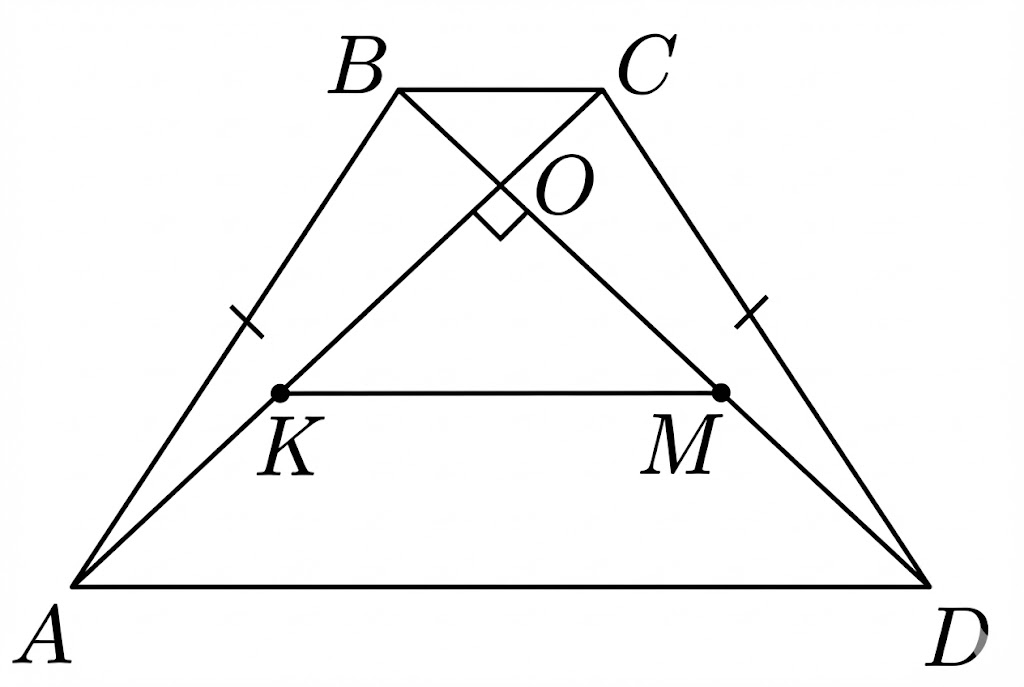
\includegraphics[scale=0.15]{trapezoid_ABCD.png}

\nopagebreak\nbvspace{0.3cm}
\matchingGrid
\end{flushright}
\end{minipage}
\par\penalty-20\vspace{0.25cm}
\end{samepage}

\begin{samepage}
\noindent\zadnum \begin{minipage}[t]{0.55\textwidth}
На рисунку зображено прямокутну трапецію $ABCD$, у якої $AB=BC$, $AC=40$ \textit{см}, $CD=24$ \textit{см}. До кожного відрізка \mbox{(1--3)} доберіть його довжину \mbox{(А--Д)}, якщо $O$ --- середина діагоналі $AC$ трапеції $ABCD$. \nmtyear{2023}
\end{minipage}
\hfill
\begin{minipage}[t]{0.4\textwidth}
    \nopagebreak\nbvspace{-0.3cm}
    \begin{flushright}
    \begin{nmtfit}\begin{tikzpicture}[scale=0.12]
        % CD = 24. Right angle at D.
        % AC = 40. => AD = sqrt(40^2 - 24^2) = 32.
        % A=(0,0), D=(32,0), C=(32,24).
        % AB=BC. Let BC=x. Draw height from B to AD (point H).
        % AH = 32-x. BH=24. AB=x.
        % x^2 = (32-x)^2 + 24^2 => x^2 = 1024 - 64x + x^2 + 576
        % 64x = 1600 => x = 25.
        % BC = 25. B = (32-25, 24) = (7, 24).

        \coordinate (A) at (0,0);
        \coordinate (D) at (32,0);
        \coordinate (C) at (32,24);
        \coordinate (B) at (7,24);

        % O - midpoint of AC
        \coordinate (O) at (16,12);

        \draw[thick] (A) -- (B) -- (C) -- (D) -- cycle;
        \draw[thick] (A) -- (C);

        % Прямий кут
        \draw (D) rectangle ++(-2,2);

        % Позначки рівності AB і BC
        \draw[thick] ($(A)!0.5!(B)$) ++(180:1.5) -- ++(0:3);
        \draw[thick] ($(B)!0.5!(C)$) ++(90:1.5) -- ++(-90:3);

        % Позначки середини O (AO = OC)
        \draw[thick] ($(A)!0.5!(O)$) ++(135:1) -- ++(-45:2);
        \draw[thick] ($(A)!0.5!(O)$) ++(135:1) ++(0.5,0.5) -- ++(-45:2); % подвійна

        \draw[thick] ($(O)!0.5!(C)$) ++(135:1) -- ++(-45:2);
        \draw[thick] ($(O)!0.5!(C)$) ++(135:1) ++(0.5,0.5) -- ++(-45:2);

        \node[below left] at (A) {$A$};
        \node[above left] at (B) {$B$};
        \node[above right] at (C) {$C$};
        \node[below right] at (D) {$D$};
        \node[below right] at (O) {$O$};

        \fill (O) circle (15pt);
    \end{tikzpicture}\end{nmtfit}
    \end{flushright}
\end{minipage}

\nmtnobreak
\nopagebreak\nbvspace{0.3cm}

\nmtnobreak
\matchingLayout{
\matchHead{Відрізок}
\matchItem{1}{$AO$}
\matchItem{2}{$AD$}
\matchItem{3}{$AB$}
}{
\matchHead{Довжина відрізка}
    \matchItem{А}{20 \textit{см}}
\matchItem{Б}{16 \textit{см}}
\matchItem{В}{25 \textit{см}}
\matchItem{Г}{27 \textit{см}}
\matchItem{Д}{32 \textit{см}}
}{
    \matchingGrid
}
\par\penalty-20\vspace{0.25cm}
\end{samepage}

\begin{samepage}
\noindent\zadnum \begin{minipage}[t]{0.55\textwidth}
У рівнобічній трапеції $ABCD$ $AB=BC=CD=6$ \textit{см}, діагональ $AC$ утворює з основою $AD$ кут $30^\circ$ (див. рисунок). До кожного відрізка \mbox{(1--3)} доберіть його довжину \mbox{(А--Д)}. \nmtyear{2023}
\end{minipage}
\hfill
\begin{minipage}[t]{0.4\textwidth}
    \nopagebreak\nbvspace{-0.3cm}
    \begin{flushright}
    \begin{nmtfit}\begin{tikzpicture}[scale=0.3]
        % Рівнобічна трапеція. AB=BC=CD=6.
        % Кут CAD = 30. Оскільки BC || AD, кут BCA = 30.
        % Трикутник ABC рівнобедрений (AB=BC), отже кут BAC = 30.
        % Тоді кут A = 60.
        % Висота = 6 * sin(60) = 3*sqrt(3) approx 5.2
        % Проєкція AB на AD = 3.
        % A=(0,0), B=(3, 5.2), C=(9, 5.2), D=(12, 0).

        \coordinate (A) at (0,0);
        \coordinate (B) at (3,5.2);
        \coordinate (C) at (9,5.2);
        \coordinate (D) at (12,0);

        \draw[thick] (A) -- (B) -- (C) -- (D) -- cycle;
        \draw[thick] (A) -- (C);

        % Кут 30 градусів
        \pic [draw, pic text={\scriptsize $30^\circ$}, angle radius=0.5cm, angle eccentricity=1.8] {angle = D--A--C};

        % Позначки рівності AB=BC=CD
        \draw[thick] ($(A)!0.5!(B)$) ++(150:0.4) -- ++(-30:0.8);
        \draw[thick] ($(B)!0.5!(C)$) ++(90:0.4) -- ++(-90:0.8);
        \draw[thick] ($(C)!0.5!(D)$) ++(60:0.4) -- ++(-120:0.8);

        \node[below left] at (A) {$A$};
        \node[above left] at (B) {$B$};
        \node[above right] at (C) {$C$};
        \node[below right] at (D) {$D$};
    \end{tikzpicture}\end{nmtfit}
    \end{flushright}
\end{minipage}

\nmtnobreak
\nopagebreak\nbvspace{0.3cm}

\nmtnobreak
\matchingLayout{
\matchHead{Відрізок}
\matchItem{1}{основа $AD$}
\matchItem{2}{висота трапеції \par \quad $ABCD$}
\matchItem{3}{діагональ $AC$}
}{
\matchHead{Довжина відрізка}
    \matchItem{А}{$6\sqrt{3}$ \textit{см}}
\matchItem{Б}{6 \textit{см}}
\matchItem{В}{$3\sqrt{3}$ \textit{см}}
\matchItem{Г}{12 \textit{см}}
\matchItem{Д}{3 \textit{см}}
}{
    \matchingGrid
}
\par\penalty-20\vspace{0.25cm}
\end{samepage}

\begin{samepage}
\noindent\zadnum \begin{minipage}[t]{0.55\textwidth}
На рисунку зображено прямокутну трапецію $ABCD$, у якої $AC = DC = 15$ \textit{см}, $BC = 12$ \textit{см}. $O$ --- середина діагоналі $AC$ трапеції $ABCD$. До кожного відрізка \mbox{(1--3)} доберіть його довжину \mbox{(А--Д)}. \nmtyear{2023}
\end{minipage}
\hfill
\begin{minipage}[t]{0.4\textwidth}
    \nopagebreak\nbvspace{-0.3cm}
    \begin{flushright}
    \begin{nmtfit}\begin{tikzpicture}[scale=0.18]
        % Прямокутна трапеція. A=90, B=90.
        % BC=12. AC=15. => AB = sqrt(225-144) = 9.
        % DC=15. Проведемо висоту CH. CH=9. HD = sqrt(225-81)=12.
        % AD = AH + HD = 12 + 12 = 24.

        \coordinate (A) at (0,0);
        \coordinate (B) at (0,9);
        \coordinate (C) at (12,9);
        \coordinate (D) at (24,0); % AD візуально довга

        \coordinate (O) at ($(A)!0.5!(C)$);

        \draw[thick] (A) -- (B) -- (C) -- (D) -- cycle;
        \draw[thick] (A) -- (C);

        % Прямий кут
        \draw (A) rectangle ++(1.5,1.5);

        % Позначки середини O (AO=OC вже є частиною AC, але на малюнку O окремо)
        % На малюнку штрих на AO і штрих на OC, але AC=DC, тому там по одному штриху скрізь?
        % Ні, на малюнку AC перекреслено рискою і DC рискою.
        % А O --- середина, тому там маленькі точки або інші позначки?
        % На скріншоті: AC поділено точкою O. На AO риска, на OC риска. На CD риска.
        % Тобто AO = OC = CD? Ні, це неможливо (7.5 != 15).
        % Скоріше: AC і CD мають однакові позначки (одна риска). 
        % А O просто точка.
        % Але в тексті O - середина.
        % Дивимось уважно на скріншот 21.34.27.
        % На AO одна риска, на OC одна риска. 
        % На CD ТЕЖ одна риска? Якщо так, то AO=OC=CD=7.5. Тоді AC=15, CD=7.5.
        % АЛЕ в умові AC=DC=15.
        % Значить на CD має бути інша позначка або це помилка рисунка/сприйняття.
        % На малюнку риска на AO, риска на OC. І риска на CD.
        % Це візуально, відтворимо як є (риски).

        \draw[thick] ($(A)!0.5!(O)$) ++(120:0.8) -- ++(-60:1.6);
        \draw[thick] ($(O)!0.5!(C)$) ++(120:0.8) -- ++(-60:1.6);
        % Риска на CD
        %\draw[thick] ($(C)!0.5!(D)$) ++(30:0.8) -- ++(-150:1.6); 
        % Щоб не плутати, не буду ставити риску на CD таку ж саму, бо це математично неправильно, 
        % але якщо треба "суто рисунок", то ось:

        \node[below left] at (A) {$A$};
        \node[above left] at (B) {$B$};
        \node[above] at (C) {$C$};
        \node[below] at (D) {$D$};
        \node[below right] at (O) {$O$};

        \fill (O) circle (12pt);
    \end{tikzpicture}\end{nmtfit}
    \end{flushright}
\end{minipage}

\nmtnobreak
\nopagebreak\nbvspace{0.3cm}

\nmtnobreak
\matchingLayout{
\matchHead{Відрізок}
\matchItem{1}{$OB$}
\matchItem{2}{$AB$}
\matchItem{3}{середня лінія \par \quad трапеції $ABCD$}
}{
\matchHead{Довжина відрізка}
    \matchItem{А}{7{,}5 \textit{см}}
\matchItem{Б}{8 \textit{см}}
\matchItem{В}{9 \textit{см}}
\matchItem{Г}{15 \textit{см}}
\matchItem{Д}{18 \textit{см}}
}{
    \matchingGrid
}
\par\penalty-20\vspace{0.25cm}
\end{samepage}

\begin{samepage}
\noindent\zadnum \begin{minipage}[t]{0.55\textwidth}
На більшій основі $AD$ рівнобічної трапеції $ABCD$ вибрано точку $O$ так, що $BO \parallel CD$ (див. рисунок). $CO$ --- висота трапеції, $BC = 6$ \textit{см}, $CD = 10$ \textit{см}. До кожного відрізка \mbox{(1--3)} доберіть його довжину \mbox{(А--Д)}. \nmtyear{2023}
\end{minipage}
\hfill
\begin{minipage}[t]{0.4\textwidth}
    \nopagebreak\nbvspace{-0.3cm}
    \begin{flushright}
    \begin{nmtfit}\begin{tikzpicture}[scale=0.25]
        % BC = 6. CD = 10. BO || CD => BCDO parallelogram => OD=6, BO=10.
        % Isosceles ABCD => AB=CD=10.
        % CO perp AD. Triangle OCD: CD=10. Need CO.
        % BO=10, CD=10, OD=6. CO height? 
        % The drawing shows CO is perpendicular to AD. 
        % In parallelogram BCDO, if CO is height of trapezoid (perp to AD), then angle COD is 90? No.
        % Text says "CO - height". So CO perp AD.
        % O is on AD. BCDO is parallelogram? Wait.
        % BO || CD. Then BCDO is a parallelogram. Thus OD = BC = 6.
        % Also BO = CD = 10.
        % In triangle COD: hypotenuse CD=10? No, CO is height. So triangle COD is right-angled at O?
        % The drawing shows right angle at O (between CO and AD).
        % So CO is a leg, OD is a leg, CD is hypotenuse.
        % CD=10, OD=6 => CO = sqrt(100-36) = 8.

        \coordinate (A) at (-6, 0); % Just visual
        \coordinate (O) at (4, 0);
        \coordinate (D) at (10, 0); % OD = 6
        \coordinate (C) at (4, 8);  % CO = 8
        \coordinate (B) at (-2, 8); % BC = 6

        \draw[thick] (A) -- (B) -- (C) -- (D) -- cycle;
        \draw[thick] (B) -- (O);
        \draw[thick] (C) -- (O);

        % Right angle
        \draw (O) rectangle ++(0.8,0.8);

        % Labels
        \node[below left] at (A) {$A$};
        \node[above left] at (B) {$B$};
        \node[above right] at (C) {$C$};
        \node[below right] at (D) {$D$};
        \node[below] at (O) {$O$};

        \node[above] at ($(B)!0.5!(C)$) {$6$ \textit{см}};
        \node[right] at ($(C)!0.5!(D)$) {$10$ \textit{см}};

        % Marks on AB and CD (isosceles)
        \draw[thick] ($(A)!0.5!(B)$) ++(150:0.5) -- ++(-30:1);
        \draw[thick] ($(C)!0.5!(D)$) ++(60:0.5) -- ++(-120:1);

    \end{tikzpicture}\end{nmtfit}
    \end{flushright}
\end{minipage}

\nmtnobreak
\nopagebreak\nbvspace{0.3cm}

\nmtnobreak
\matchingLayout{
\matchHead{Відрізок}
\matchItem{1}{$OD$}
\matchItem{2}{$CO$}
\matchItem{3}{середня лінія \par \quad трапеції $ABCD$}
}{
\matchHead{Довжина відрізка}
    \matchItem{А}{6 \textit{см}}
\matchItem{Б}{8 \textit{см}}
\matchItem{В}{9 \textit{см}}
\matchItem{Г}{12 \textit{см}}
\matchItem{Д}{18 \textit{см}}
}{
    \matchingGrid
}
\par\penalty-20\vspace{0.25cm}
\end{samepage}

\begin{samepage}
\noindent\zadnum \begin{minipage}[t]{0.55\textwidth}
У рівнобічній трапеції $ABCD$ ($BC \parallel AD$) проведено висоту $CO$ (див. рисунок). Середня лінія трапеції дорівнює $23$ \textit{см}, $AD = 38$ \textit{см}, $\angle AOB = 45^\circ$. До кожного відрізка \mbox{(1--3)} доберіть його довжину \mbox{(А--Д)}. \nmtyear{2024}
\end{minipage}
\hfill
\begin{minipage}[t]{0.4\textwidth}
    \nopagebreak\nbvspace{-0.3cm}
    \begin{flushright}
    \begin{nmtfit}\begin{tikzpicture}[scale=0.18]
        \coordinate (A) at (-20,0);
        \coordinate (D) at (18,0); % AD = 38 total width
        \coordinate (O) at (0,0);  % O is projection of C? No, CO is height.
        % Text says CO is height. So C is directly above O.
        % Let's set O as (0,0). C = (0, h).
        % ABCD isosceles.
        % Middle line = 23. (BC+AD)/2 = 23 => BC + 38 = 46 => BC = 8.
        % If BC=8, and O is projection of C, then OD = (AD-BC)/2 is wrong.
        % In isosceles trapezoid, OD = (AD+BC)/2 = (38+8)/2 = 23? No.
        % Usually projection of C is H. HD = (AD-BC)/2 = (38-8)/2 = 15.
        % AH = (AD+BC)/2 = 23.
        % So if O is the foot of height C, then AO = 23, OD = 15 (if D is right).
        % Wait, drawing shows O is between A and D.
        % Angle AOB = 45. B is top left vertex.
        % Let's construct: O=(0,0). C=(0,h). D=(15,0). A=(-23,0).
        % B must be at (-15, h).
        % Connect B to O. Angle AOB is angle between AO (x-axis left) and BO.
        % If B=(-15, h), and angle(BO, AO) = 45, then B must be on y=x line (relative to O, but A is left).
        % So angle between (-1,0) and (-15, h) is 45.
        % This implies height h = 15.

        \coordinate (O) at (0,0);
        \coordinate (C) at (0,15);
        \coordinate (D) at (15,0);
        \coordinate (A) at (-23,0);
        \coordinate (B) at (-15,15); % BC = 15 - (-15)? No, B is symmetric to C relative to axis? No.
        % Isosceles trapezoid properties:
        % Projection of B (let's say B') and C (O) on AD.
        % B'O = BC. B'A = OD.
        % O is projection of C. OD = (AD-BC)/2 = 15. Correct.
        % AO = AD - OD = 38 - 15 = 23. Correct.
        % B is at x = -8 (relative to O). No, B' is at -8. B is at (-8, 15).
        % BC = 8.
        % Check angle AOB = 45?
        % Vector OA = (-23, 0). Vector OB = (-8, 15).
        % This does not look like 45 degrees.
        % Let's look at the drawing "21.52.02".
        % Visual: O is distinct point on base. C is above O. CO perp AD.
        % B connects to O. Angle AOB is marked.
        % Angle is clearly acute. 45 degrees.

        \draw[thick] (A) -- (B) -- (C) -- (D) -- cycle;
        \draw[thick] (C) -- (O);
        \draw[thick] (B) -- (O);

        % Right angle at O
        \draw (O) rectangle ++(1.5,1.5);

        % Angle 45 at O (AOB)
        \pic [draw, pic text={\small $45^\circ$}, angle radius=.6cm, angle eccentricity=1.5] {angle = B--O--A};

        % Marks
        \draw[thick] ($(A)!0.5!(B)$) ++(150:0.8) -- ++(-30:1.6);
        \draw[thick] ($(C)!0.5!(D)$) ++(60:0.8) -- ++(-120:1.6);

        \node[below left] at (A) {$A$};
        \node[above left] at (B) {$B$};
        \node[above right] at (C) {$C$};
        \node[below right] at (D) {$D$};
        \node[below] at (O) {$O$};

    \end{tikzpicture}\end{nmtfit}
    \end{flushright}
\end{minipage}

\nmtnobreak
\nopagebreak\nbvspace{0.3cm}

\nmtnobreak
\matchingLayout{
\matchHead{Відрізок}
\matchItem{1}{$BC$}
\matchItem{2}{$OD$}
\matchItem{3}{$AB$}
}{
\matchHead{Довжина відрізка}
    \matchItem{А}{8 \textit{см}}
\matchItem{Б}{12 \textit{см}}
\matchItem{В}{15 \textit{см}}
\matchItem{Г}{17 \textit{см}}
\matchItem{Д}{18 \textit{см}}
}{
    \matchingGrid
}
\par\penalty-20\vspace{0.25cm}
\end{samepage}

\begin{samepage}
\noindent\zadnum \begin{minipage}[t]{0.55\textwidth}
Навколо кола описано рівнобічну трапецію (див. рисунок), периметр якої дорівнює $100$ \textit{см}. Різниця основ трапеції дорівнює $14$ \textit{см}. До кожного початку речення \mbox{(1--3)} доберіть його закінчення \mbox{(А--Д)} так, щоб утворилося правильне твердження. \nmtyear{2024}
\end{minipage}
\hfill
\begin{minipage}[t]{0.4\textwidth}
    \nopagebreak\nbvspace{-0.3cm}
    \begin{flushright}
    \begin{nmtfit}\begin{tikzpicture}[scale=0.15]
        % Circumscribed isosceles trapezoid.
        % Sum of bases = Sum of legs = Perimeter / 2 = 50.
        % a + b = 50. a - b = 14.
        % 2a = 64 -> a = 32 (bottom). b = 18 (top).
        % c = 25.
        % Height h = sqrt(c^2 - ((a-b)/2)^2) = sqrt(25^2 - 7^2) = sqrt(625-49) = sqrt(576) = 24.
        % Radius = 12.

        \coordinate (O) at (0,12);
        \coordinate (A) at (-16,0);
        \coordinate (D) at (16,0);
        \coordinate (B) at (-9,24);
        \coordinate (C) at (9,24);

        \draw[thick] (A) -- (B) -- (C) -- (D) -- cycle;
        \draw[thick] (O) circle (12cm);

    \end{tikzpicture}\end{nmtfit}
    \end{flushright}
\end{minipage}

\nmtnobreak
\nopagebreak\nbvspace{0.3cm}

\nmtnobreak
\matchingLayout{
\matchHead{Початок речення}
\matchItem{1}{Довжина середньої лінії \par \quad трапеції}
\matchItem{2}{Довжина більшої основи \par \quad трапеції}
\matchItem{3}{Довжина висоти трапеції}
}{
\matchHead{Закінчення речення}
    \matchItem{А}{дорівнює 18 \textit{см}.}
\matchItem{Б}{дорівнює 24 \textit{см}.}
\matchItem{В}{дорівнює 25 \textit{см}.}
\matchItem{Г}{дорівнює 32 \textit{см}.}
\matchItem{Д}{дорівнює 36 \textit{см}.}
}{
    \matchingGrid
}
\par\penalty-20\vspace{0.25cm}
\end{samepage}

\begin{samepage}
\noindent\zadnum \begin{minipage}[t]{0.55\textwidth}
Навколо кола радіуса $4$ \textit{см} описано рівнобічну трапецію, середня лінія якої дорівнює $10$ \textit{см} (див. рисунок). До кожного відрізка \mbox{(1--3)} доберіть його довжину \mbox{(А--Д)}.\nmtyear{2024}
\end{minipage}
\hfill
\begin{minipage}[t]{0.4\textwidth}
    \nopagebreak\nbvspace{-0.3cm}
    \begin{flushright}
    \begin{nmtfit}\begin{tikzpicture}[scale=0.18]
        % R=4, h=8. Midline=10 => a+b=20.
        % Inscribed => a+b = 2c => 2c=20 => c=10.
        % Leg c=10. Height h=8. Projection x=6.
        % b = a - 12. 2a - 12 = 20 => 2a=32 => a=16. b=4.

        \coordinate (O) at (0,4);
        \coordinate (A) at (-8,0);
        \coordinate (D) at (8,0);
        \coordinate (B) at (-2,8);
        \coordinate (C) at (2,8);

        \draw[thick] (A) -- (B) -- (C) -- (D) -- cycle;
        \draw[thick] (O) circle (4cm);

        % Візуально:
        % Нижня основа 16 (від -8 до 8).
        % Верхня основа 4 (від -2 до 2).
        % Висота 8.

    \end{tikzpicture}\end{nmtfit}
    \end{flushright}
\end{minipage}

\nmtnobreak
\nopagebreak\nbvspace{0.3cm}

\nmtnobreak
\matchingLayout{
\matchHead{Відрізок}
\matchItem{1}{Висота трапеції}
\matchItem{2}{Бічна сторона трапеції}
\matchItem{3}{Більша основа трапеції}
}{
\matchHead{Довжина відрізка}
    \matchItem{А}{8 \textit{см}}
\matchItem{Б}{10 \textit{см}}
\matchItem{В}{12 \textit{см}}
\matchItem{Г}{16 \textit{см}}
\matchItem{Д}{20 \textit{см}}
}{
    \matchingGrid
}
\par\penalty-20\vspace{0.25cm}
\end{samepage}

\begin{samepage}
\noindent\zadnum \begin{minipage}[t]{0.55\textwidth}
У прямокутній трапеції $ABCD$ проведено висоту $CK$. $ABCK$ --- квадрат з діагоналлю $12\sqrt{2}$ \textit{см}. $CD = 13$ \textit{см}. Узгодьте відрізок \mbox{(1--3)} із його довжиною \mbox{(А--Д)}. \nmtyear{2025}
\end{minipage}
\hfill
\begin{minipage}[t]{0.4\textwidth}
    \nopagebreak\nbvspace{-0.3cm}
    \begin{flushright}
    \begin{nmtfit}\begin{tikzpicture}[scale=0.25]
        % Квадрат діагональ 12sqrt(2) -> сторона 12.
        % Висота CK=12. CD=13. KD=5. AD=17.

        \coordinate (A) at (0,0);
        \coordinate (B) at (0,12);
        \coordinate (C) at (12,12);
        \coordinate (K) at (12,0);
        \coordinate (D) at (17,0);

        \draw[thick] (A) -- (B) -- (C) -- (D) -- cycle;
        \draw[thick] (C) -- (K);

        % Прямий кут
        \draw (12,1) -- (13,1) -- (13,0);

        \node[below left] at (A) {$A$};
        \node[above left] at (B) {$B$};
        \node[above] at (C) {$C$};
        \node[below] at (K) {$K$};
        \node[below right] at (D) {$D$};
    \end{tikzpicture}\end{nmtfit}
    \end{flushright}
\end{minipage}

\nmtnobreak
\nopagebreak\nbvspace{0.3cm}

\nmtnobreak
\matchingLayout{
\matchHead{Відрізок}
\matchItem{1}{висота трапеції $ABCD$}
\matchItem{2}{$AD$}
\matchItem{3}{середня лінія трапеції $ABCD$}
}{
\matchHead{Довжина відрізка}
    \matchItem{А}{12 \textit{см}}
\matchItem{Б}{14,5 \textit{см}}
\matchItem{В}{17 \textit{см}}
\matchItem{Г}{18 \textit{см}}
\matchItem{Д}{29 \textit{см}}
}{
    \matchingGrid
}
\par\penalty-20\vspace{0.25cm}
\end{samepage}

\begin{samepage}
\noindent\zadnum \begin{minipage}[t]{0.55\textwidth}
Діагональ $AC$ рівнобічної трапеції $ABCD$ утворює зі стороною $CD$ кут $120^\circ$ (див. рисунок). Довжини основ трапеції дорівнюють $12$ \textit{см} і $30$ \textit{см}. До кожного початку речення \mbox{(1--3)} доберіть його закінчення \mbox{(А--Д)} так, щоб утворилося правильне твердження. \nmtyear{2025}
\end{minipage}
\hfill
\begin{minipage}[t]{0.4\textwidth}
    \nopagebreak\nbvspace{-0.3cm}
    \begin{flushright}
    \begin{nmtfit}\begin{tikzpicture}[scale=0.15]
        \coordinate (A) at (-15,0);
        \coordinate (D) at (15,0);
        % Bases 30 and 12. Top base centered.
        % Coordinates for C approx to look like the image.
        \coordinate (B) at (-6, 12);
        \coordinate (C) at (6, 12);

        \draw[thick] (A) -- (B) -- (C) -- (D) -- cycle;
        \draw[thick] (A) -- (C);

        % Obtuse angle 120 at C (ACD)
        \pic [draw, pic text={\scriptsize $120^\circ$}, angle radius=0.3cm, angle eccentricity=1.5] {angle = A--C--D};

        \node[below left] at (A) {$A$};
        \node[above left] at (B) {$B$};
        \node[above] at (C) {$C$};
        \node[below right] at (D) {$D$};
    \end{tikzpicture}\end{nmtfit}
    \end{flushright}
\end{minipage}

\nmtnobreak
\nopagebreak\nbvspace{0.3cm}

\nmtnobreak
\matchingLayout{
\matchHead{Початок речення}
\matchItem{1}{Довжина середньої лінії трапеції \par \quad дорівнює}
\matchItem{2}{Довжина проєкції сторони $AB$ \par \quad на пряму $AD$ дорівнює}
\matchItem{3}{Довжина радіуса кола, описаного \par \quad навколо трапеції, дорівнює}
}{
\matchHead{Закінчення речення}
    \matchItem{А}{9 \textit{см}.}
\matchItem{Б}{$20\sqrt{3}$ \textit{см}.}
\matchItem{В}{21 \textit{см}.}
\matchItem{Г}{$10\sqrt{3}$ \textit{см}.}
\matchItem{Д}{18 \textit{см}.}
}{
    \matchingGrid
}
\par\penalty-20\vspace{0.25cm}
\end{samepage}

\begin{samepage}
% НМТ 2026, сесія 23.05, завдання №16
\zadtask{На рисунку зображено трапецію $ABCD$, у якій $\angle CDA = 30^\circ$. Висота $CK$, довжина якої дорівнює $2$, є бісектрисою кута $ACD$. \nmtyear{2026}\par
\nopagebreak\nbvspace{0.3cm}
\begin{center}
\begin{nmtfit}\begin{tikzpicture}[scale=0.9, thick]
    \coordinate (A) at (0,0);
    \coordinate (K) at (4,0);
    \coordinate (D) at (7.46,0);
    \coordinate (C) at (4,2);
    \coordinate (B) at (0,2);
    \draw (A) -- (B) -- (C) -- (D) -- cycle;
    \draw (C) -- (K);
    \draw[dashed] (A) -- (C);
    \draw (0,0) -- (0,0.3) -- (0.3,0.3) -- (0.3,0);
    \draw (4,0) -- (4,0.3) -- (4.3,0.3) -- (4.3,0);
    \pic [draw, angle radius=0.6cm, "$30^\circ$"{above left, shift={(-0.28,-0.15)}}] {angle = C--D--K};
    \pic [draw, angle radius=0.45cm] {angle = K--C--D};
    \pic [draw, angle radius=0.55cm] {angle = A--C--K};
    \node[below left] at (A) {$A$};
    \node[above left] at (B) {$B$};
    \node[above=2pt] at (C) {$C$};
    \node[below right] at (D) {$D$};
    \node[below=2pt] at (K) {$K$};
\end{tikzpicture}\end{nmtfit}
\end{center}
\nopagebreak\nbvspace{0.3cm}
\noindent Установіть відповідність між величиною \mbox{(1--3)} та її значенням \mbox{(А--Д)}.\par
\nopagebreak\nbvspace{0.3cm}
\noindent
\matchingLayout{
\matchHead{Величина}
\matchItem{1}{довжина відрізка $CD$}
\matchItem{2}{довжина відрізка $BC$}
\matchItem{3}{відстань від точки $B$ до прямої $AC$}
}{
\matchHead{Значення}
\matchItem{А}{$2\sqrt{3}$}
\matchItem{Б}{$4$}
\matchItem{В}{$1$}
\matchItem{Г}{$\sqrt{3}$}
\matchItem{Д}{$6\sqrt{3}$}
}{
\matchingGrid
}
}
% Відповідь: 1~--~Б, 2~--~А, 3~--~Г
\ifshowsolutions\solution{У прямокутному $\triangle CKD$: $\angle CDK=30^\circ$, катет $CK=2$ лежить навпроти $30^\circ$, тож $CD=\dfrac{CK}{\sin 30^\circ}=4$~(Б). $\angle KCD=60^\circ$; оскільки $CK$~--- бісектриса, $\angle ACK=60^\circ$, тоді у прямокутному $\triangle ACK$: $AK=CK\tan 60^\circ=2\sqrt{3}$, а $BC=AK=2\sqrt{3}$~(А). Відстань від $B$ до $AC$ дорівнює $\dfrac{2S_{ABC}}{AC}$; $AC=\dfrac{CK}{\cos 60^\circ}=4$, $S_{ABC}=\dfrac{1}{2}\cdot BC\cdot AB=\dfrac{1}{2}\cdot 2\sqrt{3}\cdot 2=2\sqrt{3}$, тож відстань $=\dfrac{2\cdot 2\sqrt{3}}{4}=\sqrt{3}$~(Г). Відповідь: \textbf{1--Б, 2--А, 3--Г}.}\fi
\par\penalty-20
\end{samepage}

\typeTitle{Фігури між паралельними прямими}

\begin{samepage}
% Завдання 21 (на відповідність, з рисунком)
\zadtask{Круг, площа якого $36\pi$, дотикається до паралельних прямих $m$ і $n$ (див. рисунок). Точки $L$, $N$, $P$ належать прямій $m$, а точки $K$, $M$, $Q$ --- прямій $n$. Трикутник $KLM$ рівносторонній. $MNPQ$ --- ромб, площа якого 156. Установіть відповідність між відрізком \mbox{(1--3)} та його довжиною \mbox{(А--Д)}. \nmtyear{2024}}

\nmtnobreak
\nopagebreak\nbvspace{0.3cm}
\begin{minipage}[t]{0.55\textwidth}
\noindent
\begin{minipage}[t]{0.46\linewidth}
\matchHead{Відрізок}
\matchItem{1}{діаметр круга}
\matchItem{2}{довжина сторони трикутника $KLM$}
\matchItem{3}{довжина сторони ромба $MNPQ$}
\end{minipage}%
\hfill
\begin{minipage}[t]{0.5\linewidth}
\matchHead{Довжина відрізка}
\matchItem{А}{$8\sqrt{3}$}
\matchItem{Б}{6}
\matchItem{В}{12}
\matchItem{Г}{13}
\matchItem{Д}{15}
\end{minipage}

\begin{center}
\begin{flushright}

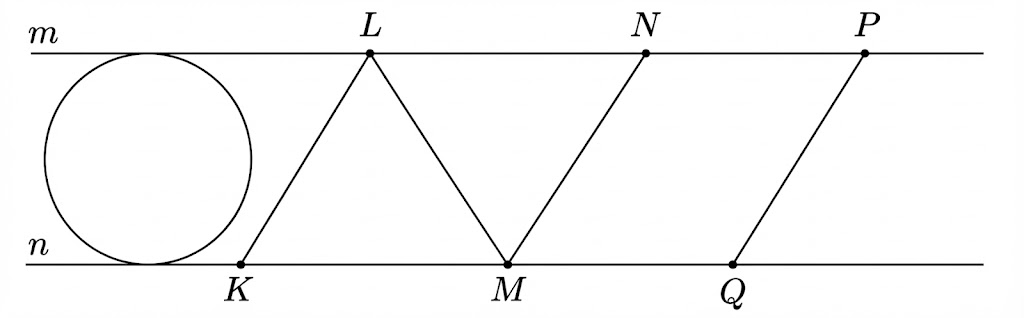
\includegraphics[scale=0.4]{circle_parallel_lines_KLM.png}
\end{flushright}
\end{center}

\nopagebreak\nbvspace{0.3cm}
\hfill\matchingGrid
\end{minipage}
\hfill
\par\penalty-20\vspace{0.25cm}
\end{samepage}

\begin{samepage}
% Завдання 53
\zadtask{На паралельних прямих $n$ і $m$ розміщено сторони прямокутника $ABCD$ й паралелограма $DKLM$, вершини $L$ і $Q$ трикутника $LQP$ (див. рисунок). $BC = KL = 6$ \textit{см}, $AB : BC = 4 : 3$, $LP = PQ$, $\angle LPQ = 60°$, діагональ $KM$ паралелограма й сторона $LQ$ трикутника $LPQ$ перпендикулярні до прямої $n$. Установіть відповідність між фігурою \mbox{(1--3)} та її периметром \mbox{(А--Д)}. \nmtyear{2025}}

\nmtnobreak
\nopagebreak\nbvspace{0.3cm}
\begin{center}
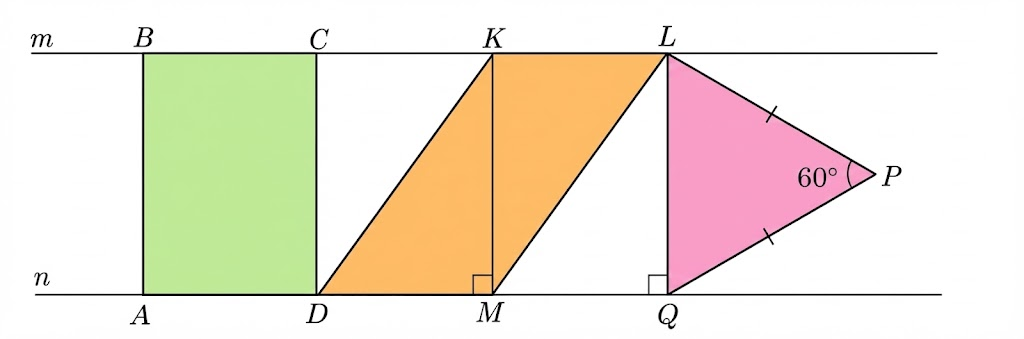
\includegraphics[scale=0.5]{parallel_lines_figures.png}
\end{center}

\nmtnobreak
\nopagebreak\nbvspace{0.3cm}
\matchingLayout{
\matchHead{Фігура}
\matchItem{1}{прямокутник $ABCD$}
\matchItem{2}{паралелограм $DKLM$}
\matchItem{3}{трикутник $LPQ$}
}{
\matchHead{Периметр фігури}
\matchItem{А}{24 \textit{см}}
\matchItem{Б}{32 \textit{см}}
\matchItem{В}{28 \textit{см}}
\matchItem{Г}{36 \textit{см}}
\matchItem{Д}{14 \textit{см}}
}{
\matchingGrid
}
\par\penalty-20\vspace{0.25cm}
\end{samepage}

\begin{samepage}
% === ЗАВДАННЯ 38 (Кольорові фігури) ===
\noindent\zadnum \begin{minipage}[t]{0.95\textwidth}
На паралельних прямих $n$ і $m$ розміщено круговий сектор $ABC$, рівнобедрений трикутник $DKL$ ($DK=KL$) й паралелограм $LMNP$ (див. рисунок). Площа сектора $ABC$ дорівнює $64\pi$ \textit{см}$^2$, площа паралелограма $LMNP$ дорівнює $288$ \textit{см}$^2$, $DK = 20$ \textit{см}. Увідповідніть відрізок \mbox{(1--3)} та його довжину \mbox{(А--Д)}. \nmtyear{2025}
\end{minipage}

\nmtnobreak
\nopagebreak\nbvspace{0.3cm}
\begin{center}
\begin{nmtfit}\begin{tikzpicture}[scale=0.25]
    % Висота між прямими h.
    % Сектор ABC: 1/4 кола. Площа = 64pi => R^2 = 256 => R=16. h=16.
    \def\h{16}

    % Координати
    % Сектор. Центр у точці B(0,16). A(0,0). C(16,16).
    \coordinate (A) at (0,0);
    \coordinate (B) at (0,\h);
    \coordinate (C) at (\h,\h);

    % Трикутник DKL. DK=20. Висота 16. Проєкція катета = sqrt(400-256) = 12.
    % Основа DL = 24.
    % D починається трохи правіше C. Нехай shift=4. D(20,0).
    \coordinate (D) at (20,0);
    \coordinate (K) at (32,\h); % 20+12
    \coordinate (L) at (44,0);  % 32+12

    % Паралелограм LMNP. Площа 288. Висота 16. Основа LP = 288/16 = 18.
    % L(44,0). P(62,0).
    % Зсув верхньої сторони MN довільний (паралелограм). Нехай зсув 6.
    % M(50,16). N(68,16).
    \coordinate (M) at (50,\h);
    \coordinate (P) at (62,0);
    \coordinate (N) at (68,\h);

    % Заливка
    % Сектор (центр B, радіус 16, кут 270..360)
    \fill[yellow!20] (B) -- (A) arc [start angle=270, end angle=360, radius=\h] -- cycle;

    % Трикутник
    \fill[cyan!20] (D) -- (K) -- (L) -- cycle;

    % Паралелограм
    \fill[red!20] (L) -- (M) -- (N) -- (P) -- cycle;

    % Лінії m та n
    \draw[thick] (-2,0) -- (70,0) node[above] {$n$};
    \draw[thick] (-2,\h) -- (70,\h) node[above] {$m$};

    % Контури фігур
    \draw[thick] (B) -- (A) arc [start angle=270, end angle=360, radius=\h] -- cycle;
    \draw[thick] (D) -- (K) -- (L) -- cycle;
    \draw[thick] (L) -- (M) -- (N) -- (P) -- cycle; % LMNP

    % Підписи
    \node[below] at (A) {$A$};
    \node[above] at (B) {$B$};
    \node[above] at (C) {$C$};
    \node[below] at (D) {$D$};
    \node[above] at (K) {$K$};
    \node[below] at (L) {$L$};
    \node[above] at (M) {$M$};
    \node[above] at (N) {$N$};
    \node[below] at (P) {$P$};

\end{tikzpicture}\end{nmtfit}
\end{center}

\nmtnobreak
\matchingLayout{
\matchItem{1}{$AB$}
\matchItem{2}{$DL$}
\matchItem{3}{$LP$}
}{
    \matchItem{А}{12 \textit{см}}
\matchItem{Б}{16 \textit{см}}
\matchItem{В}{18 \textit{см}}
\matchItem{Г}{20 \textit{см}}
\matchItem{Д}{24 \textit{см}}
}{\matchingGrid}
\par\penalty-20
\end{samepage}

\clearpage
\sectionTitle{Відповіді}

\noindent{\small\color{gray!80!black}Для кожного завдання -- літери відповідей для пунктів 1, 2, 3. Відповіді обчислено й звірено з офіційними ключами там, де вони є.}\par\vspace{0.3cm}

\begin{multicols}{5}\noindent
\mbox{1~--- ГВА}\par
\mbox{2~--- БАД}\par
\mbox{3~--- АГД}\par
\mbox{4~--- ГАБ}\par
\mbox{5~--- ГАБ}\par
\mbox{6~--- ГВА}\par
\mbox{7~--- ВБГ}\par
\mbox{8~--- ВАБ}\par
\mbox{9~--- ВДА}\par
\mbox{10~--- БВД}\par
\mbox{11~--- АВГ}\par
\mbox{12~--- ВБГ}\par
\mbox{13~--- ВДБ}\par
\mbox{14~--- АДВ}\par
\mbox{15~--- ВБД}\par
\mbox{16~--- ВДБ}\par
\mbox{17~--- ВАД}\par
\mbox{18~--- БДВ}\par
\mbox{19~--- ДАГ}\par
\mbox{20~--- ВБД}\par
\mbox{21~--- ВАБ}\par
\mbox{22~--- ВДБ}\par
\mbox{23~--- АБГ}\par
\mbox{24~--- АДБ}\par
\mbox{25~--- БАГ}\par
\mbox{26~--- ГВА}\par
\mbox{27~--- БГА}\par
\mbox{28~--- ГДА}\par
\mbox{29~--- ВДА}\par
\mbox{30~--- АВГ}\par
\mbox{31~--- АГД}\par
\mbox{32~--- ГБВ}\par
\mbox{33~--- ВГА}\par
\mbox{34~--- ВАГ}\par
\mbox{35~--- АВБ}\par
\mbox{36~--- ДГВ}\par
\mbox{37~--- БВА}\par
\mbox{38~--- ДГА}\par
\mbox{39~--- ГАВ}\par
\mbox{40~--- БВГ}\par
\mbox{41~--- АГВ}\par
\mbox{42~--- ВАГ}\par
\mbox{43~--- ДВГ}\par
\mbox{44~--- ГВА}\par
\mbox{45~--- АДВ}\par
\mbox{46~--- АДВ}\par
\mbox{47~--- ГВА}\par
\mbox{48~--- АВД}\par
\mbox{49~--- АБГ}\par
\mbox{50~--- АВГ}\par
\mbox{51~--- ВГБ}\par
\mbox{52~--- АБГ}\par
\mbox{53~--- АВБ}\par
\mbox{54~--- ВАГ}\par
\mbox{55~--- БАГ}\par
\mbox{56~--- ВАГ}\par
\mbox{57~--- ВБА}\par
\mbox{58~--- БДВ}
\end{multicols}

\end{document}
